\documentclass[UTF8,a4paper,12pt]{ctexart}
\usepackage[margin=2.5cm]{geometry}
\usepackage{graphicx}
\usepackage{booktabs}
\usepackage{longtable}
\usepackage{tabularx}
\usepackage{array}
\usepackage{calc}
\usepackage{amsmath}
\usepackage{amssymb}
\usepackage{enumitem}
\usepackage{caption}
\usepackage{fancyhdr}
\usepackage{float}
\usepackage[hidelinks]{hyperref}
\usepackage{xcolor}

\setcounter{tocdepth}{3}
\setlength{\parindent}{2em}
\setlength{\parskip}{0.35em}
\setlist{itemsep=0.2em, topsep=0.3em, parsep=0pt, partopsep=0pt}
\renewcommand{\arraystretch}{1.2}
\graphicspath{{src/assets/}{assets/}}
\captionsetup{font=small,labelfont=bf,position=bottom}
\captionsetup[table]{position=top,skip=6pt}
\pagestyle{fancy}
\fancyhf{}
\fancyfoot[C]{\thepage}
\renewcommand{\headrulewidth}{0pt}
\renewcommand{\footrulewidth}{0pt}
\newcolumntype{L}[1]{>{\raggedright\arraybackslash}p{#1}}
\newcolumntype{C}[1]{>{\centering\arraybackslash}p{#1}}
\newenvironment{threelongtable}[1]{%
  \setlength\LTleft{\fill}%
  \setlength\LTright{\fill}%
  \renewcommand{\arraystretch}{1.2}%
  \small
  \begin{longtable}{#1}%
}{%
  \end{longtable}%
}
\newcommand{\coverfield}[2]{%
  {\zihao{4}\noindent\makebox[6em][l]{\heiti#1：}%
   \underline{\makebox[\dimexpr\textwidth-6em\relax][l]{\strut\heiti #2}}\par}%
}
\newcommand{\quickpreviewtitle}{%
  \par\bigskip
  \phantomsection
	{\centering\zihao{4}\textbf{快速预览简介}\par}%
  \addcontentsline{toc}{section}{快速预览简介}%
  \medskip
}

\title{基于RISC-V指令集的CPU设计\\竞业达分赛区决赛测评报告}
\author{队伍编号：CICC1004252\\团队名称：和溢位}
\date{}

\begin{document}
\begin{titlepage}
  \centering
  
\includegraphics[width=0.35\textwidth]{image1.png}\par\vspace{1.2cm}
  {\zihao{2}\bfseries 第十届\\全国大学生集成电路创新创业大赛\par}
  \vspace*{\fill}
  \begin{minipage}{\textwidth}
    \raggedright
    \setlength{\parindent}{0pt}
    \coverfield{报告类型}{分赛区决赛测评报告}
    \vspace{0.45cm}
    \coverfield{参赛杯赛}{``竞业达"企业命题}
    \vspace{0.45cm}
    \coverfield{作品名称}{基于RISC-V指令集的CPU设计}
    \vspace{0.45cm}
    \coverfield{队伍编号}{CICC1004252}
    \vspace{0.45cm}
    \coverfield{团队名称}{和溢位}
    \vspace{2cm}
  \end{minipage}
\end{titlepage}

\tableofcontents
\clearpage

\part[上板验证报告]{RISC-V CPU上板验证报告}
\setcounter{section}{0}

\quickpreviewtitle

上板验证使用竞业达 FPGA 数字孪生平台 Xilinx Kintex-7 XC7K325T-2FFG900 器件，在 Vivado 2024.2 下完成综合、实现和 bitstream 生成；
\textbf{280 MHz 时钟约束下 WNS 为 +0.050 ns}，无建立时间违例，满足时序要求。

280 MHz 时钟下，官方 \texttt{src0}、\texttt{src1}、\texttt{src2} 以及新增的
\texttt{withoutMext}、\texttt{withMext} 均完成数字孪生平台远程烧录和运行验证，行为正确；
运行时间分别为 \textbf{7.101 s、7.047 s、9.233 s、3.890 s、2.020 s}。
其中 \texttt{src0}、\texttt{src1}、\texttt{src2} 相对于赛题给出的 50 MHz 单周期参考设计，
性能倍率分别为 \textbf{$\times$4.00、$\times$3.70、$\times$4.00}。


\newpage

\section{验证平台说明}

本项目最终验证平台为竞业达 FPGA 数字孪生平台，对应开发板核心器件为 Xilinx Kintex-7 XC7K325T-2FFG900。板端可观察资源主要包括 LED 阵列、八位数码管以及平台状态指示区，能够满足本项目对程序运行结果可视化展示的需要。

\subsection{下载/烧录工具版本}

bitstream 生成阶段使用 Vivado 2024；远程下载与板级观察阶段使用竞业达数字孪生平台配套的自动烧录工具。工程完成综合、实现和比特流生成后，通过平台加载设备、选择 bit 文件并执行远程烧录。

\subsection{上电与平台显示验证说明}

本项目的板级外设连接基于竞业达官方提供的 FPGA 模板完成，LED、数码管和 UART 等接口均已在模板顶层中预先接好。本项目在此基础上完成 CPU 顶层与板级显示逻辑的对接，其中 UART 主要用于与孪生数字平台进行通信，并非本次上板验证中面向用户的主要交互输出通道；本次验证结果主要通过平台运行状态、LED 阵列显示和数码管显示进行判断。

具体实现上，本项目将 LED 与数码管显示值作为设备寄存器相关输出接入自定义 Top 顶层，其中数码管显示值通过模板提供的显示驱动模块转换为可直接驱动数码管的控制信号，再与 LED 显示信息一并送入板级控制路径，由孪生数字平台完成状态同步与显示。

在实际测试过程中，完成 bitstream 烧录并打开数字孪生平台后，若平台运行状态显示正常，且 LED、数码管显示结果与测试程序预期一致，则判定该测试用例通过。

\section{测试用例说明}

\subsection{指令程序例程}

本次上板验证采用官方工程提供的 \texttt{src0}、\texttt{src1}、\texttt{src2}，以及新测试程序
\texttt{withoutMext}、\texttt{withMext}。五组程序均已完成比特流生成，
并在竞业达数字孪生平台上完成烧录与运行验证。

\subsection{上板运行流程说明}

\begin{enumerate}[label=\arabic*）]
  \item 在 Vivado 2024.2 中打开工程，完成综合、实现并生成 bitstream。
  \item 配置孪生平台网络连接环境，启动数字孪生平台并加载可用设备。
  \item 在烧录界面中选择生成的 bit 文件，执行远程烧录。
  \item 烧录成功后打开孪生平台界面，观察``运行状态''、``数据运行正常''、``串口运行正常''等状态提示。
  \item 记录 LED 阵列和八位数码管显示结果，并与测试用例预期进行比对。
  \item 依次完成五组程序的上板验证。
\end{enumerate}

\section{验证结果}

\subsection{数字孪生运行截图/照片}

下列截图为分赛区决赛工程在竞业达数字孪生平台上的实际运行结果。

\begin{figure}[H]
  \centering
  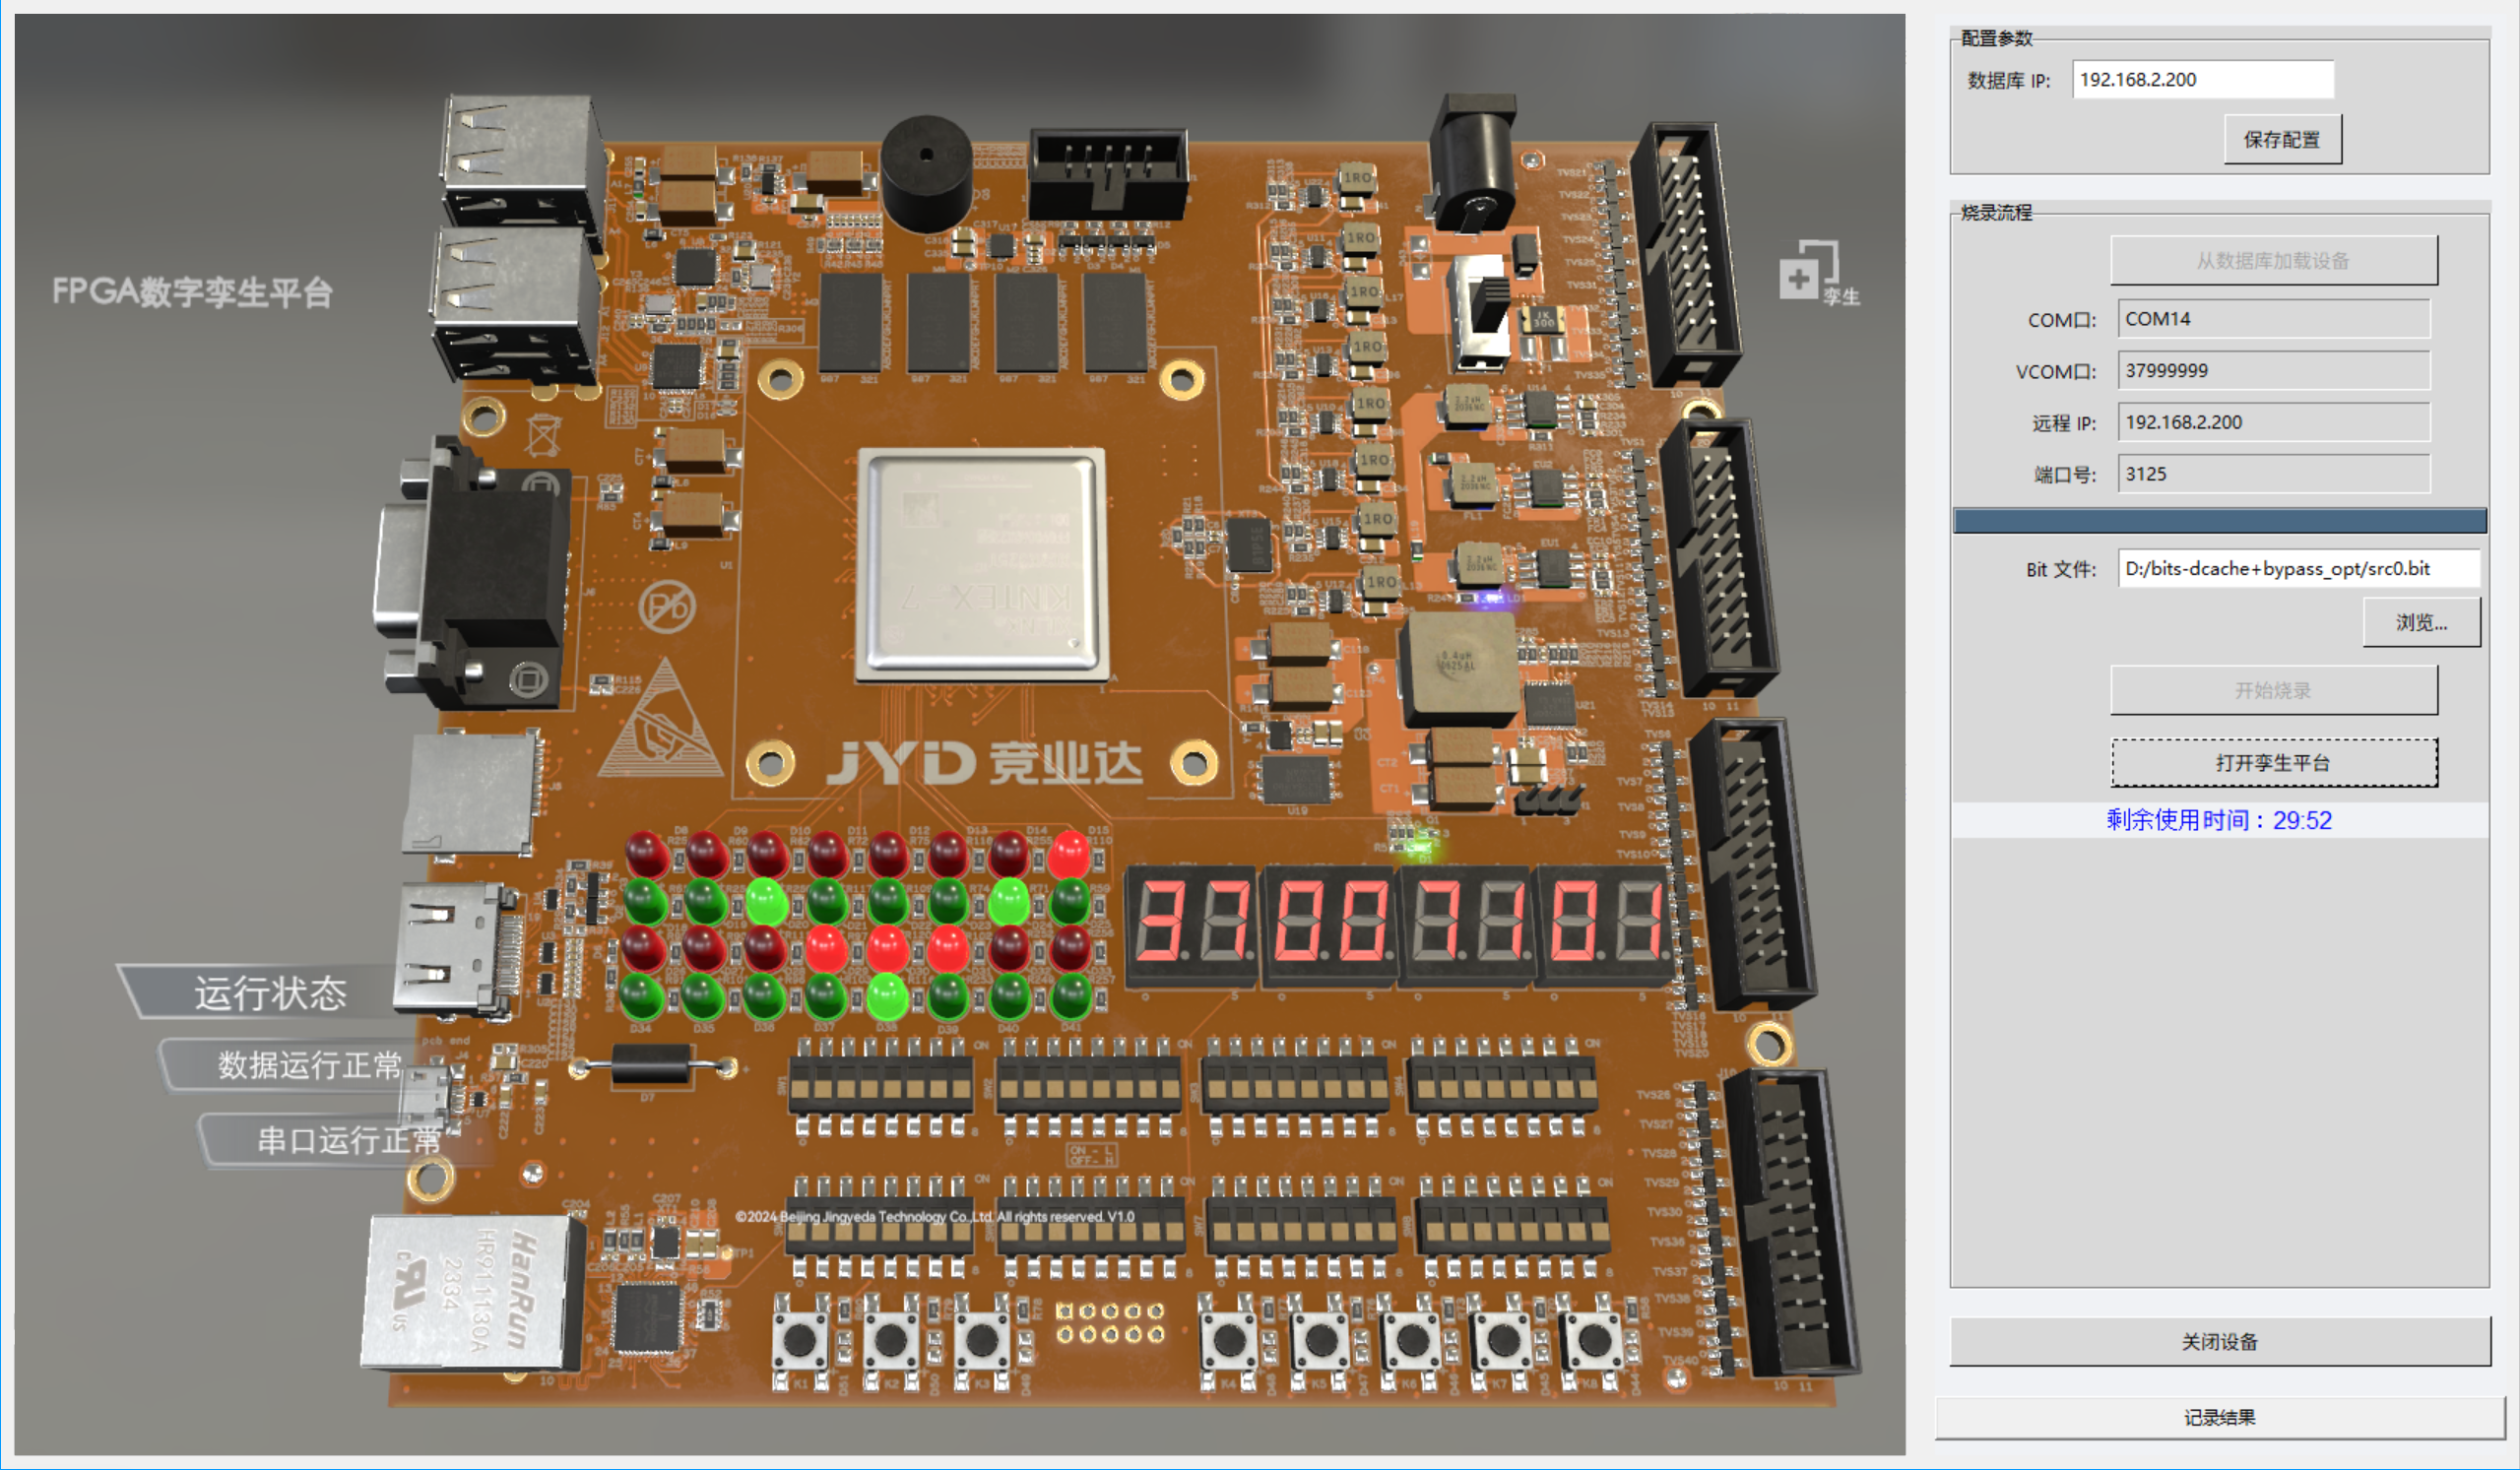
\includegraphics[width=\linewidth]{board/src0.png}
  \caption{src0 上板测试结果（7.101s）}
\end{figure}

\begin{figure}[H]
  \centering
  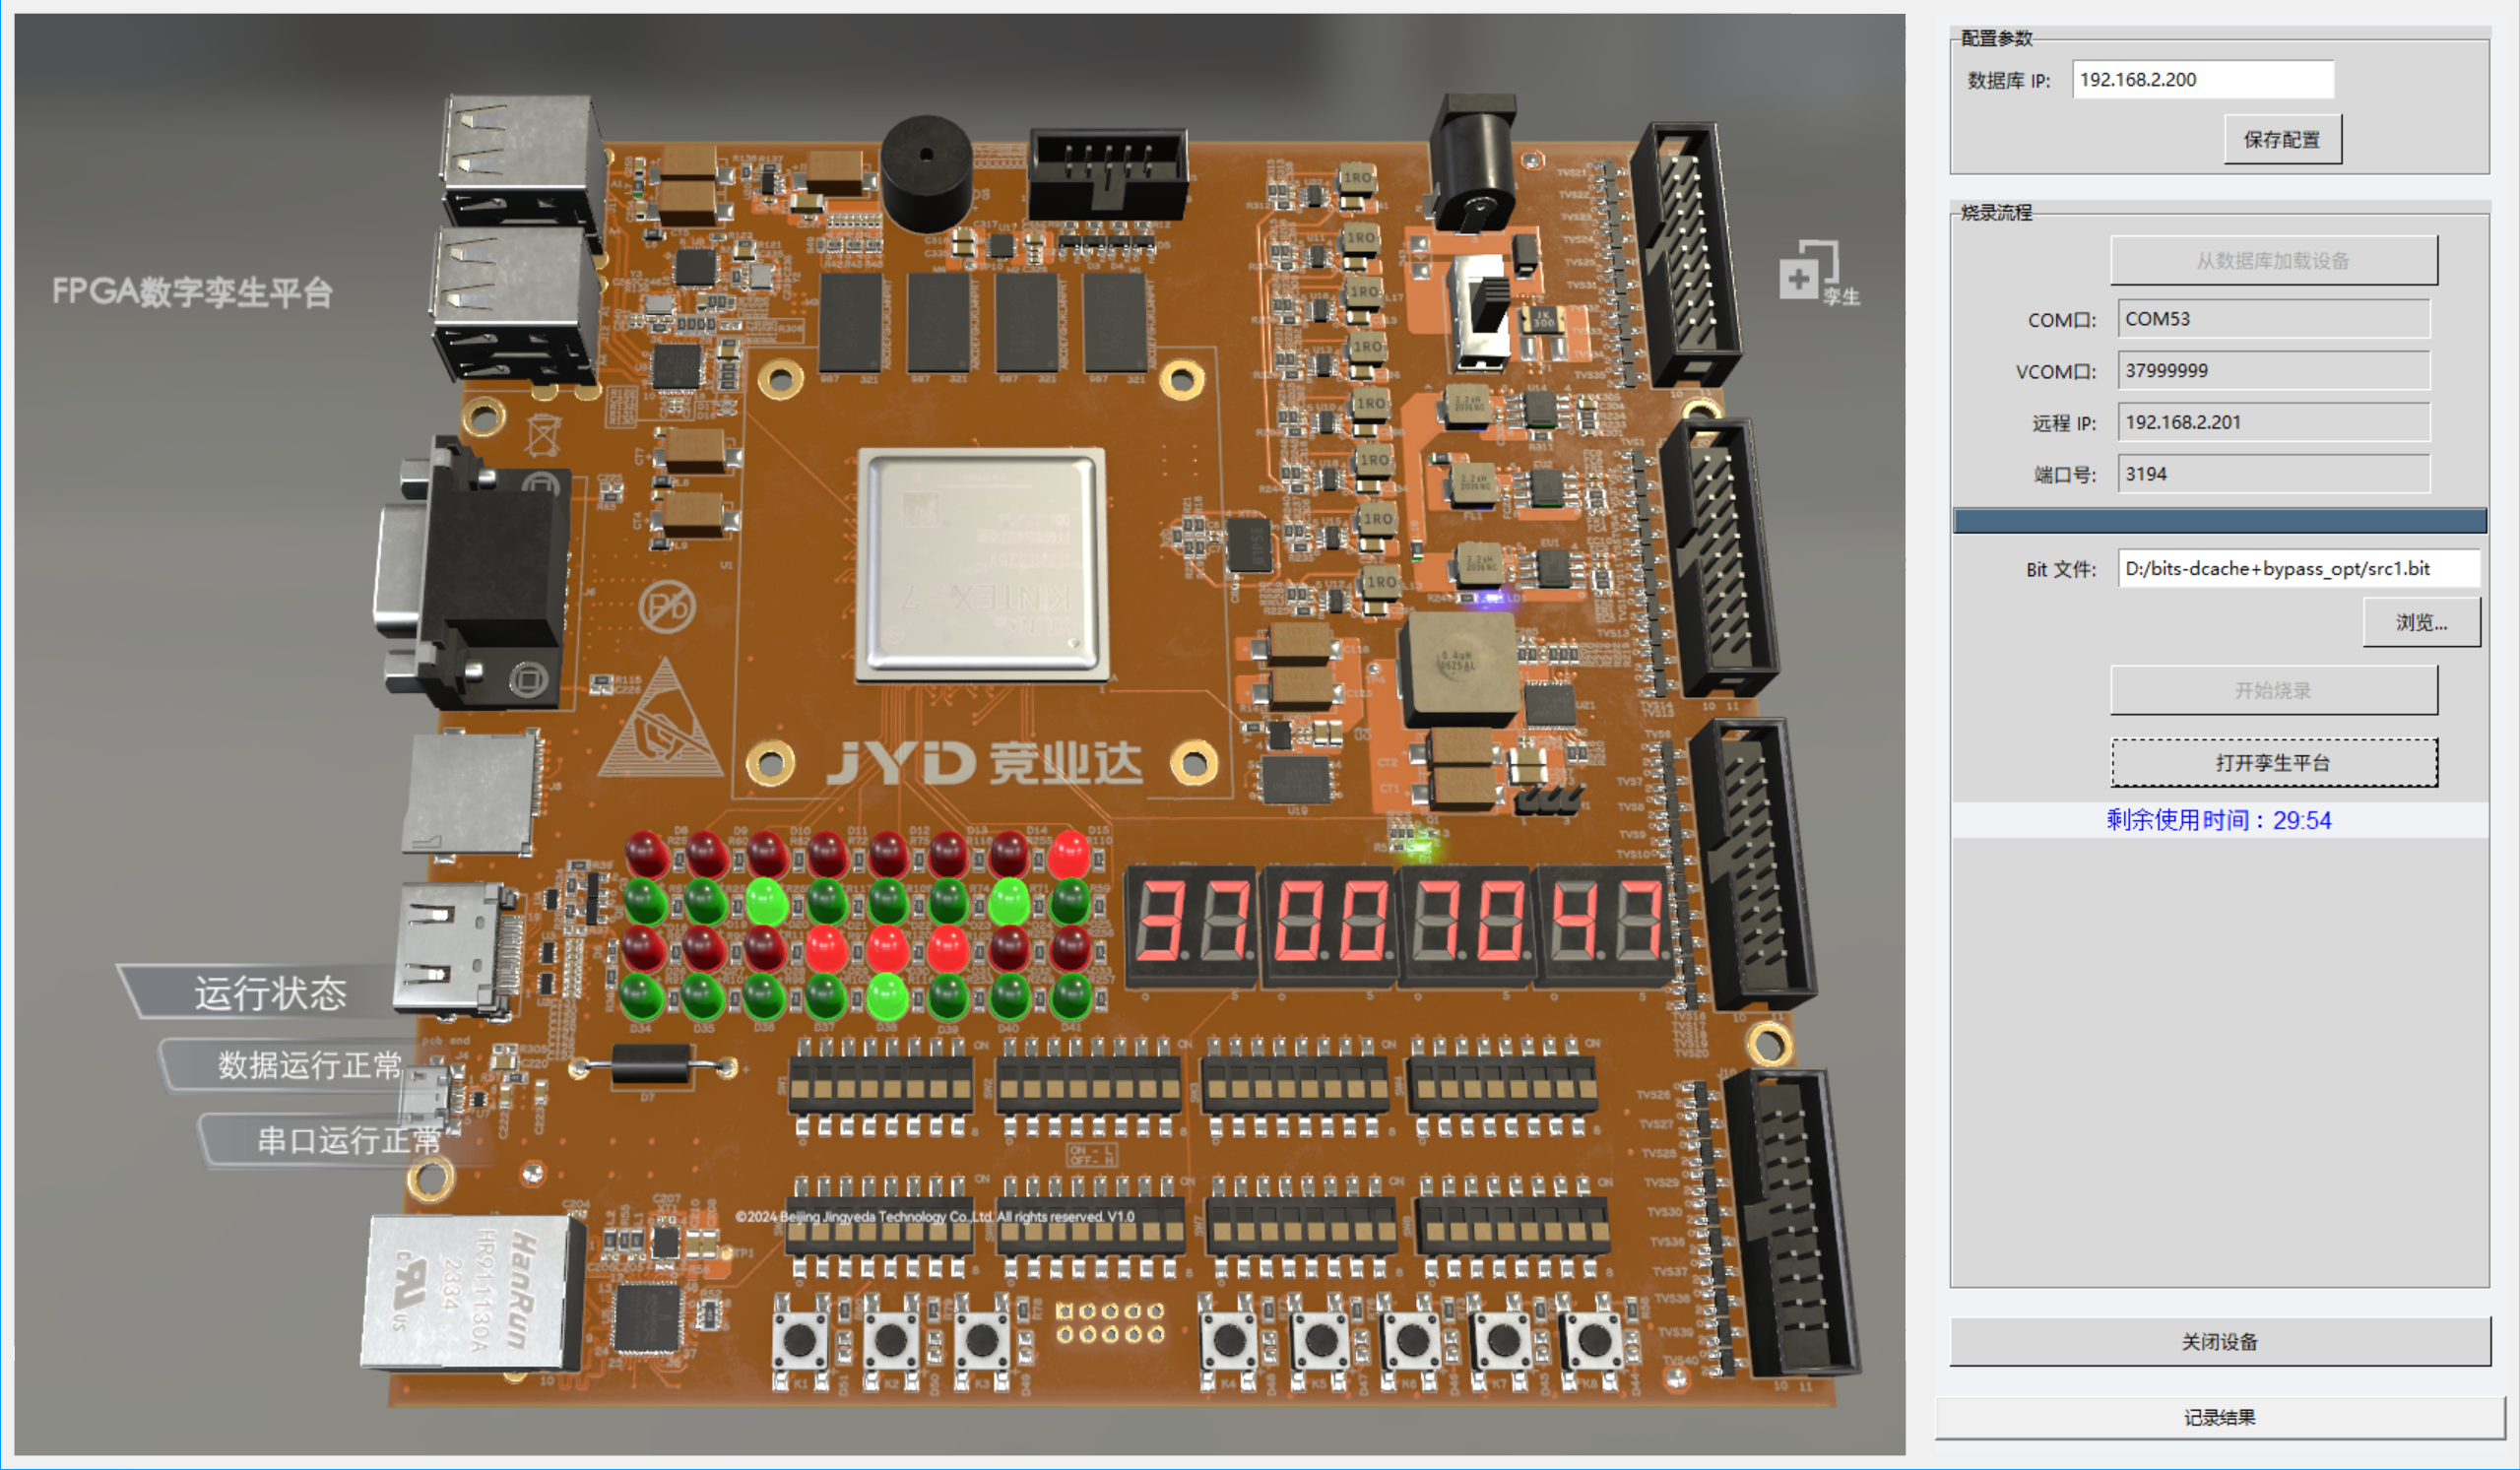
\includegraphics[width=\linewidth]{board/src1.png}
  \caption{src1 上板测试结果（7.047s）}
\end{figure}

\begin{figure}[H]
  \centering
  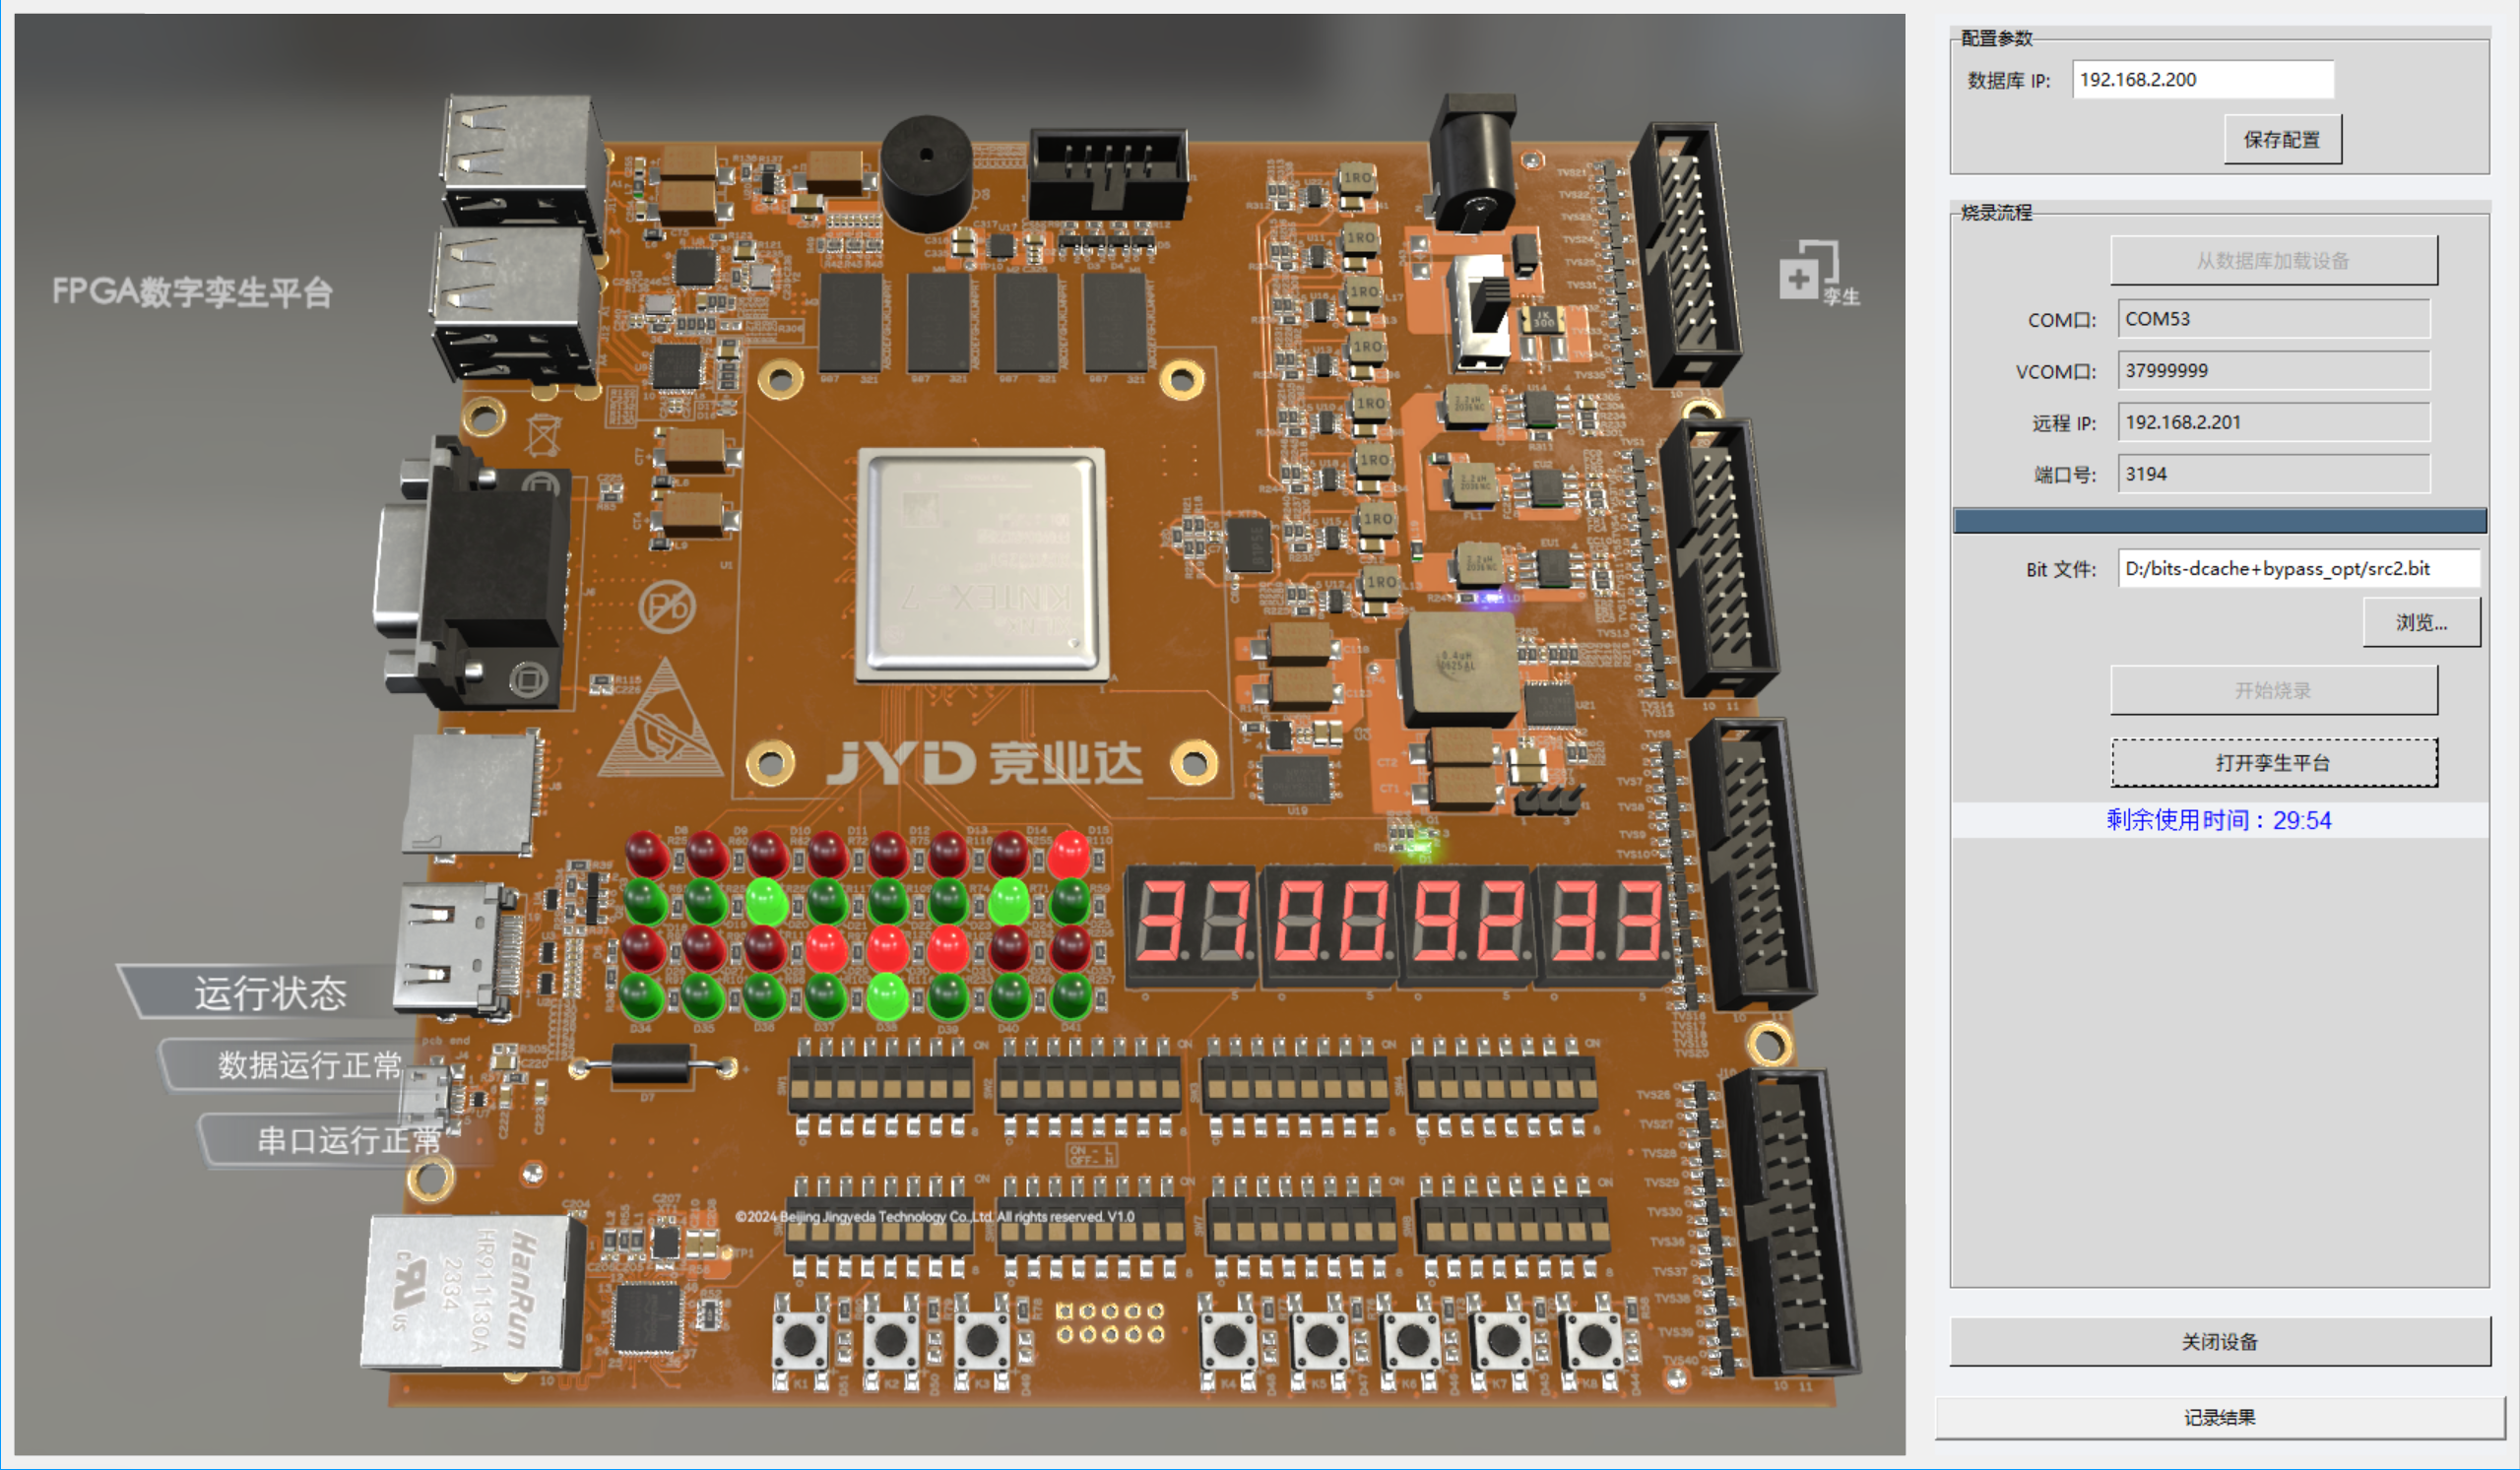
\includegraphics[width=\linewidth]{board/src2.png}
  \caption{src2 上板测试结果（9.233s）}
\end{figure}

\begin{figure}[H]
  \centering
  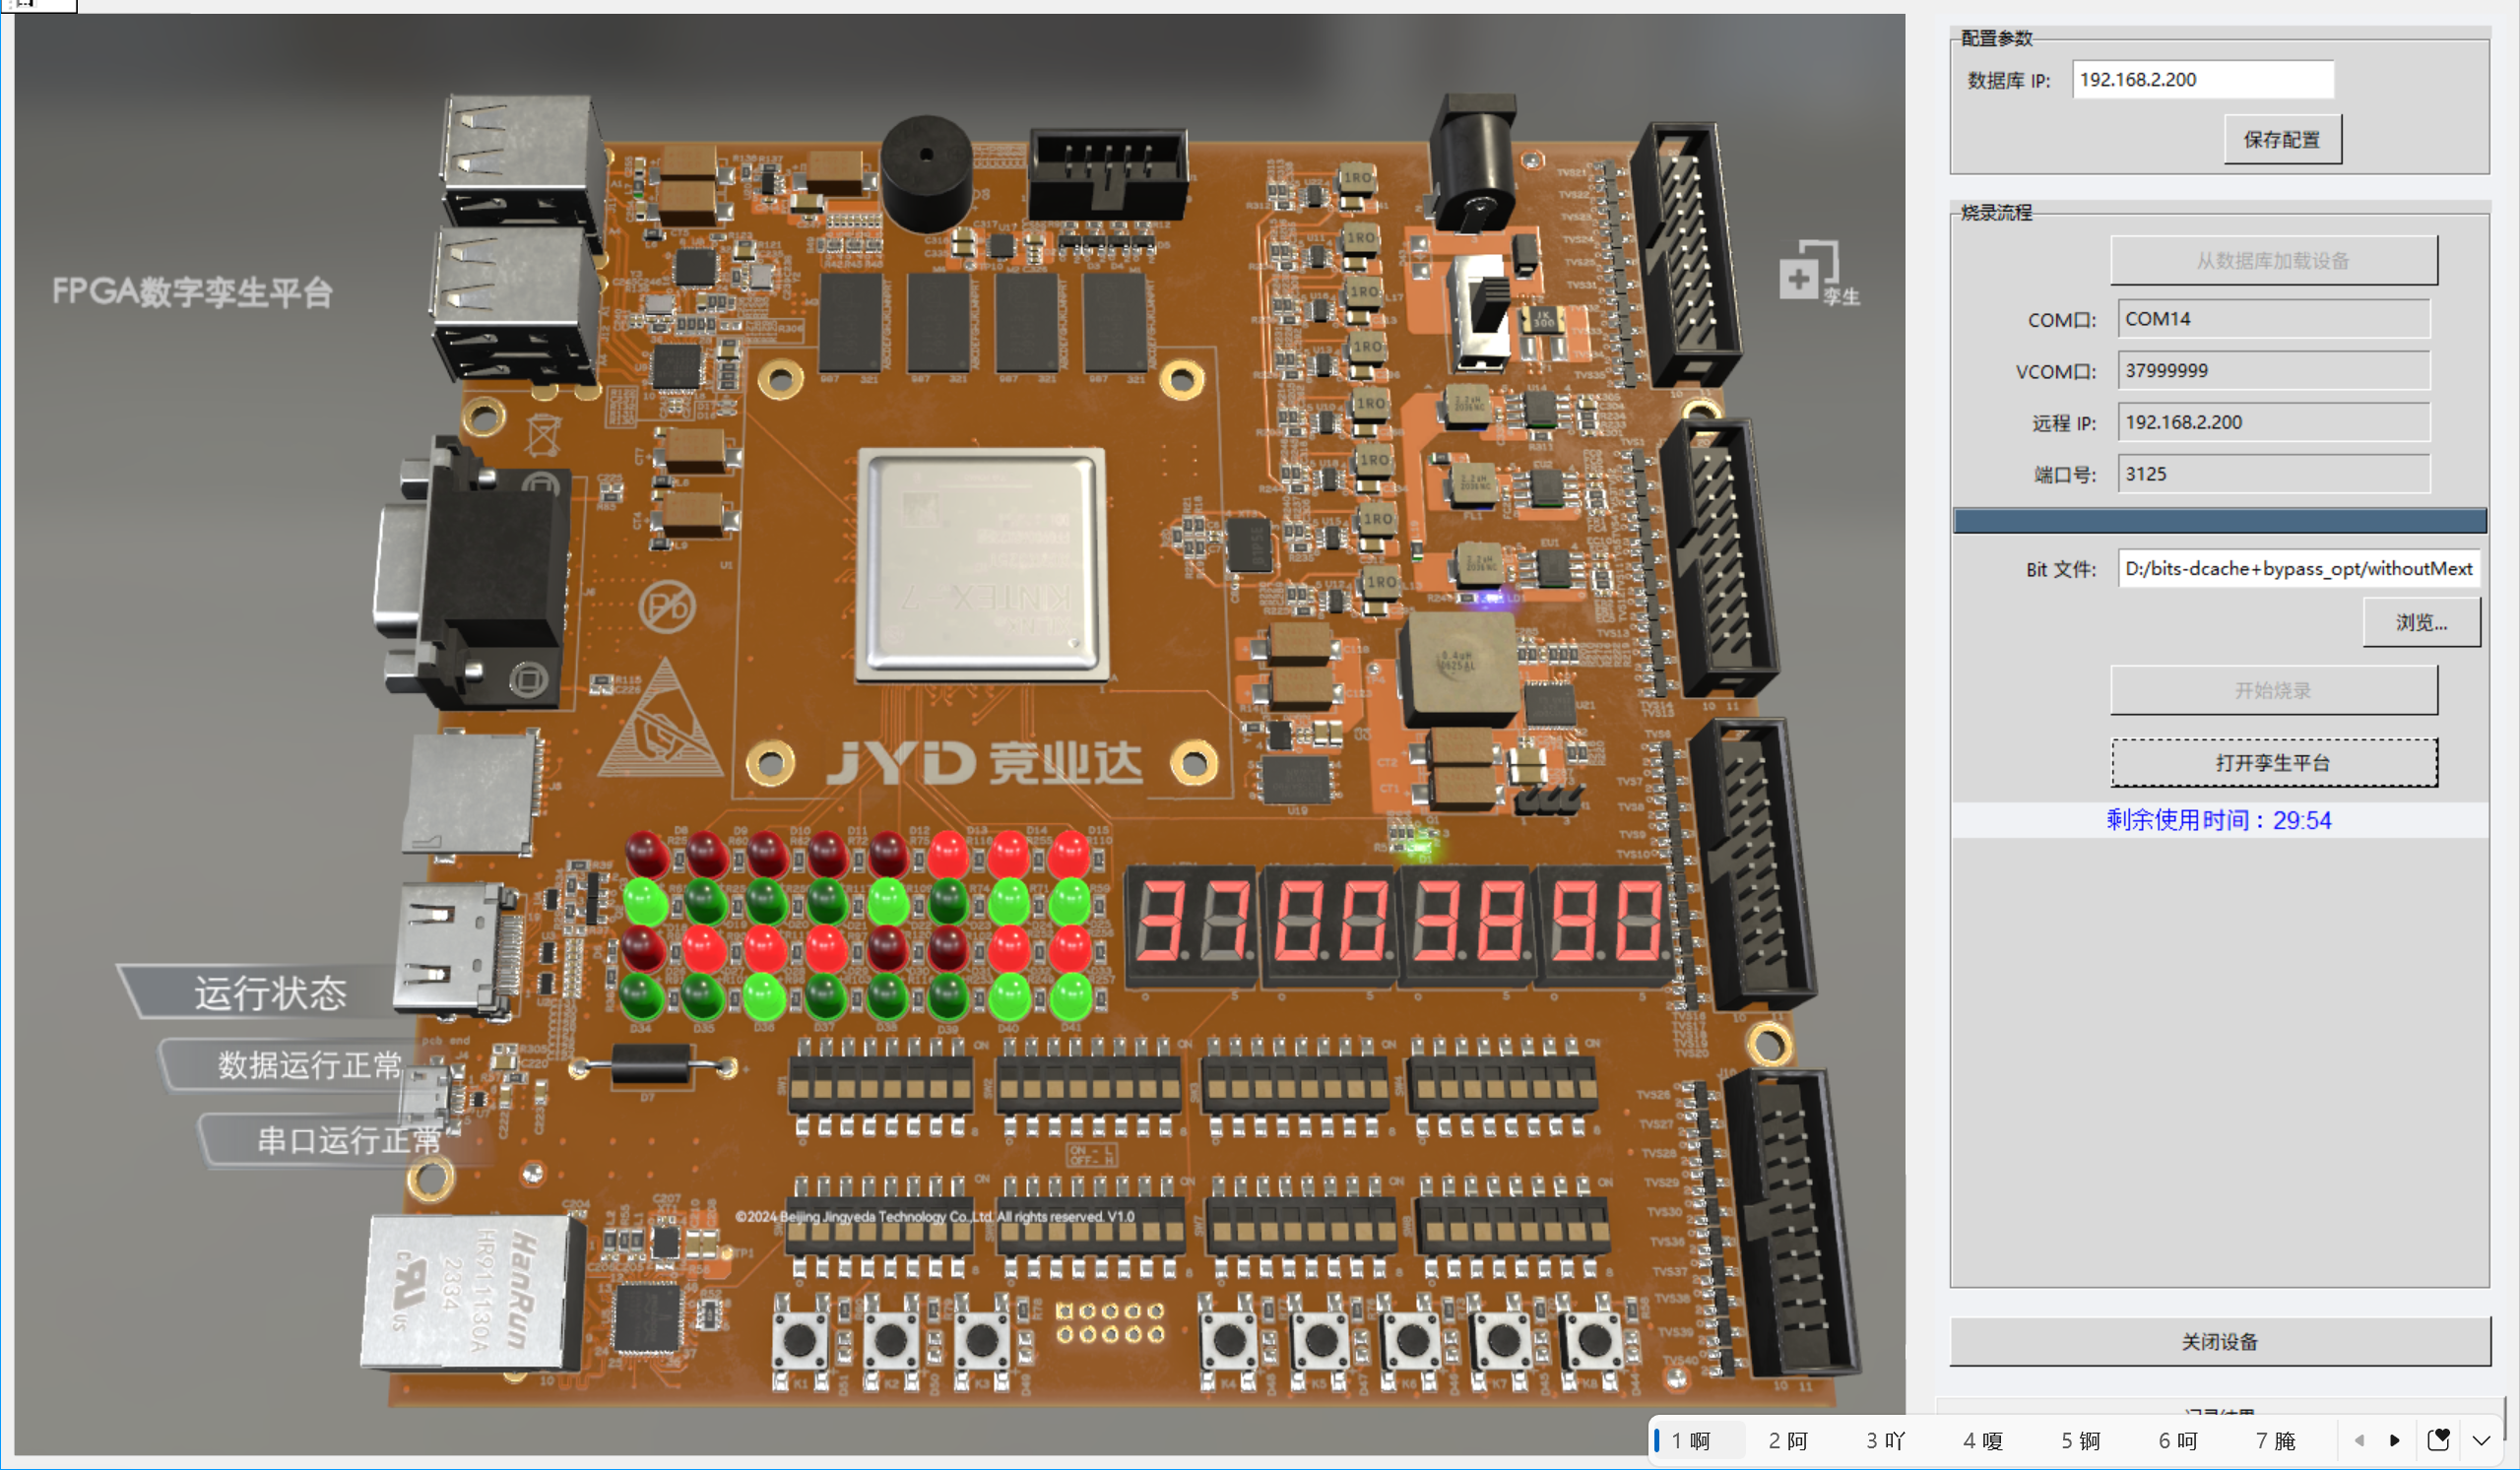
\includegraphics[width=\linewidth]{board/withoutMext.png}
  \caption{withoutMext 上板测试结果（3.890s）}
\end{figure}

\begin{figure}[H]
  \centering
  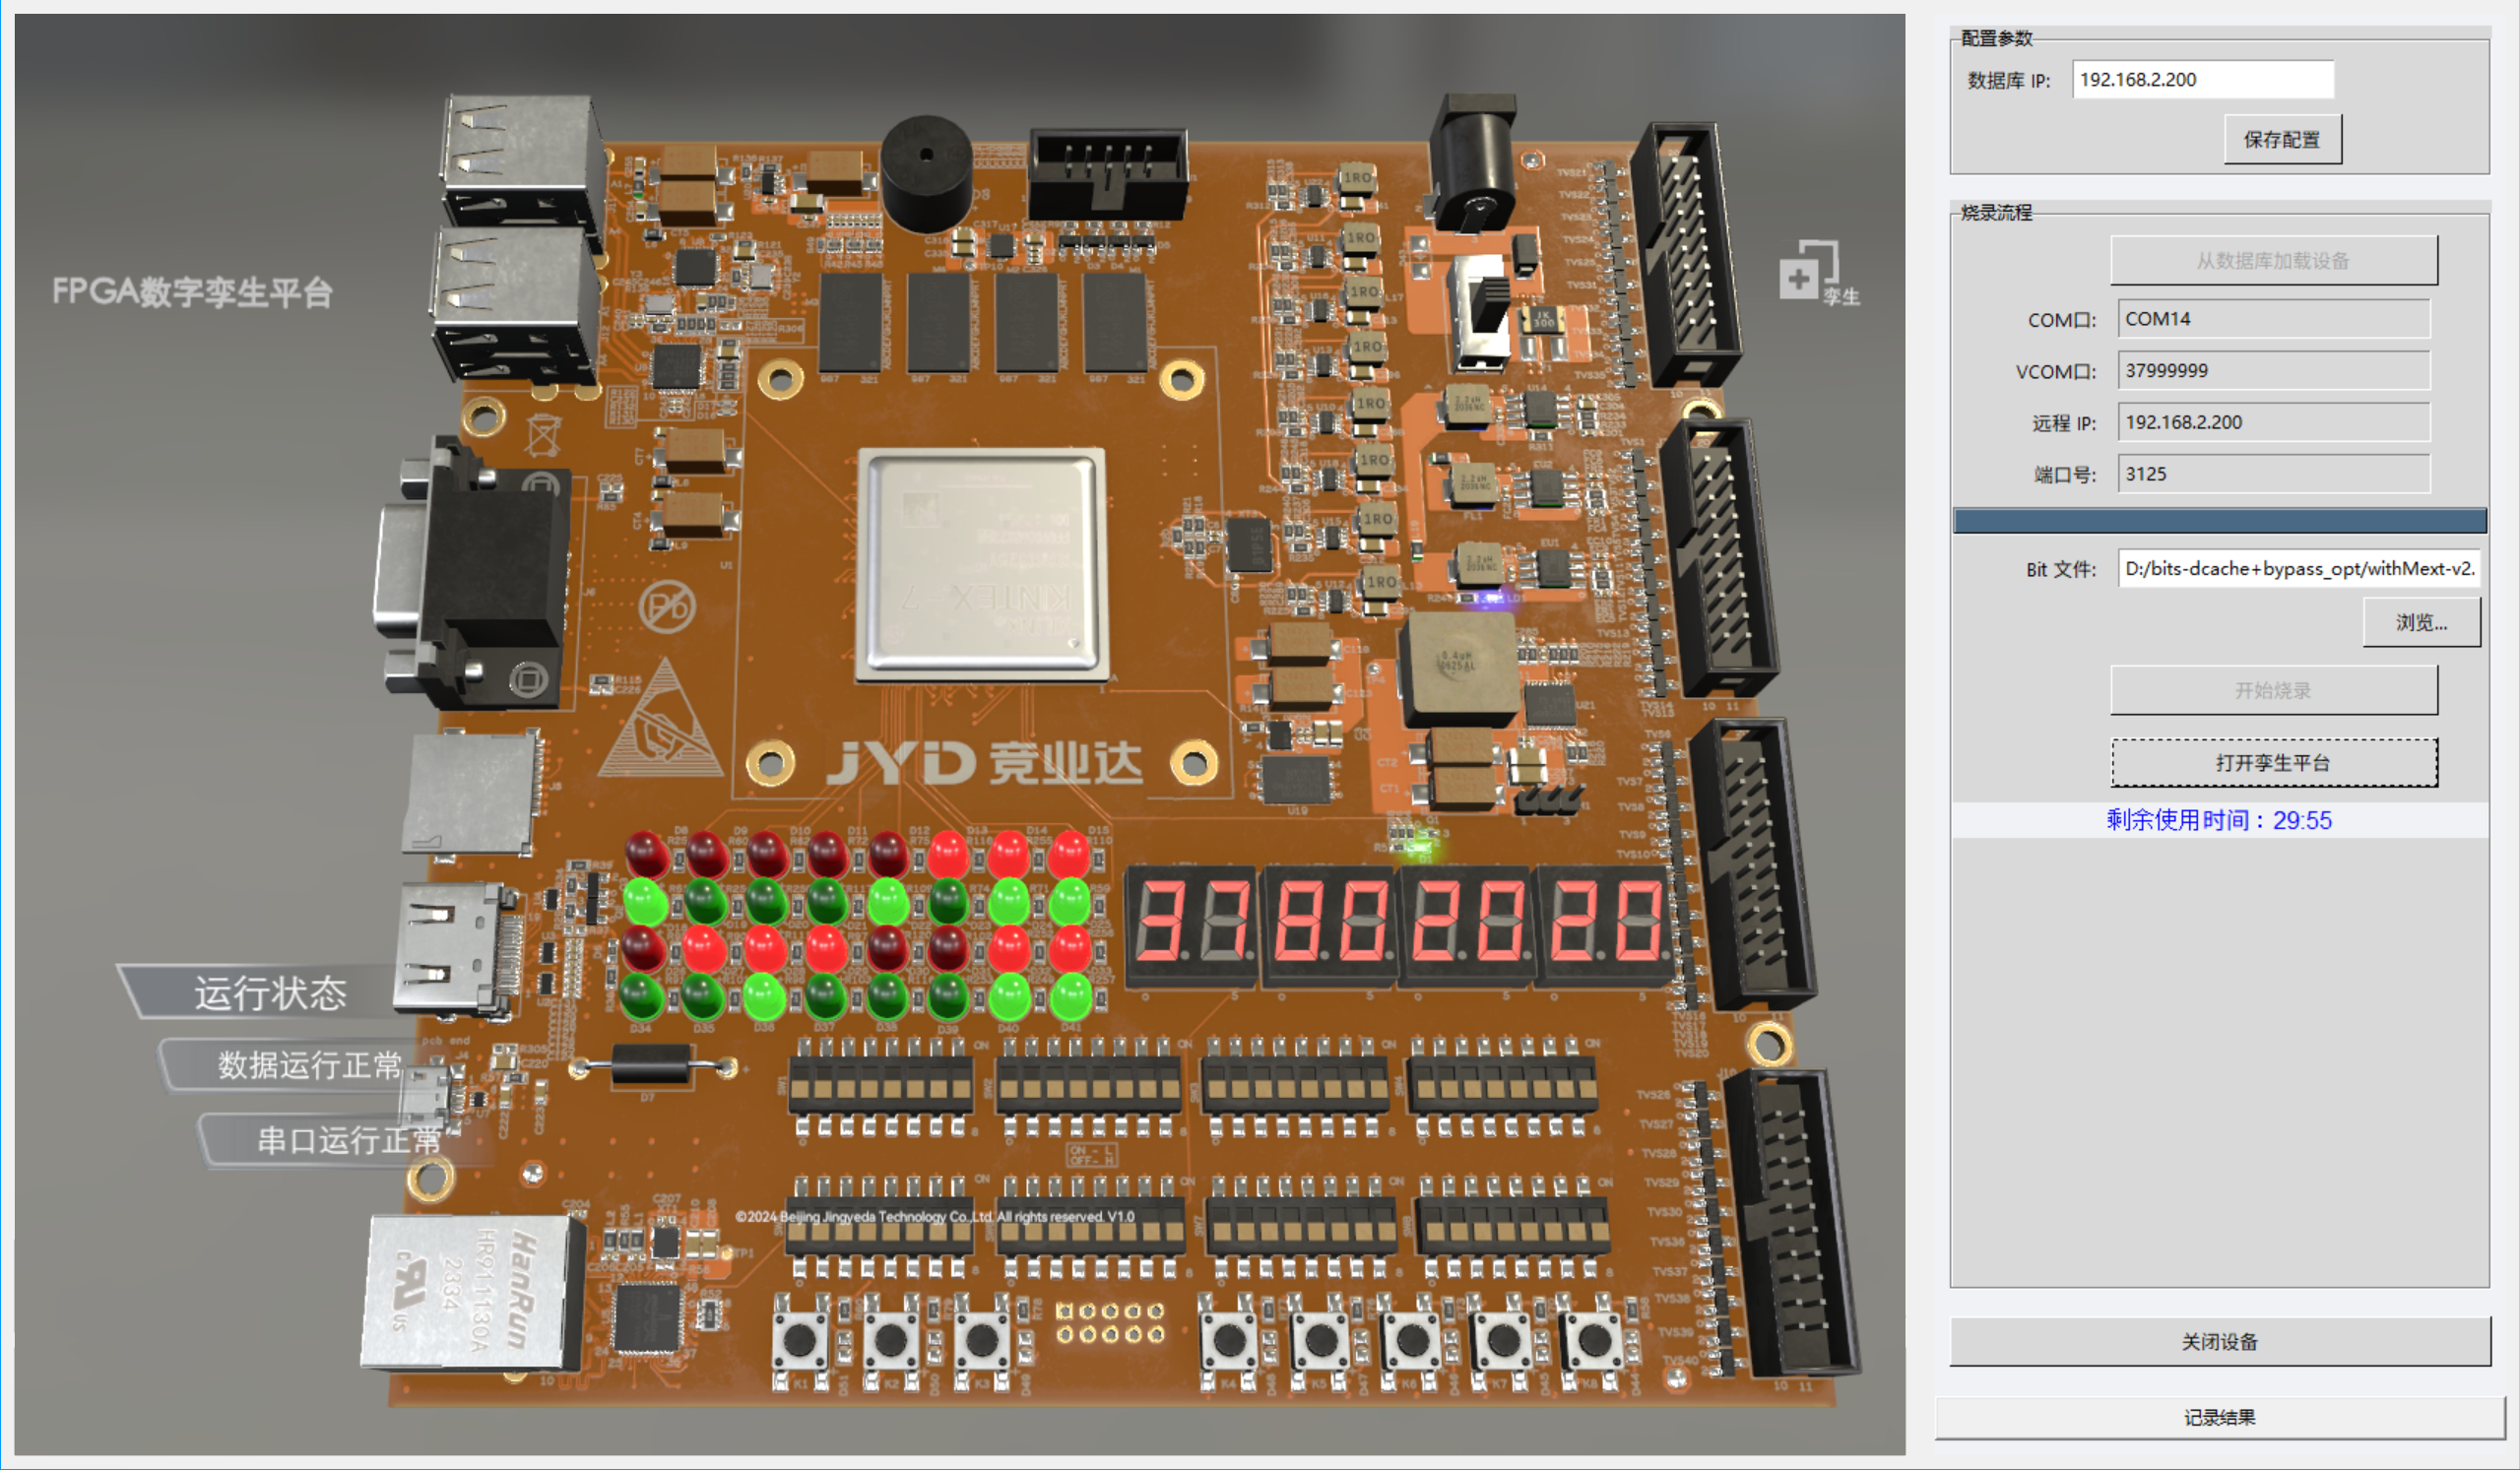
\includegraphics[width=\linewidth]{board/withMext.png}
  \caption{withMext 上板测试结果（2.020s）}
\end{figure}

从上述截图可以看到，平台已经成功加载开发板并打开孪生界面，状态栏显示运行正常；同时 LED 阵列与数码管给出了各自的显示结果，说明对应程序在板端完成执行且运行正确。

\subsection{280 MHz 时序收敛说明}

工程在 Vivado 2024.2 中采用 Performance\_WLBlockPlacement 作为 implementation strategy 进行布局布线优化。

\begin{figure}[H]
  \centering
  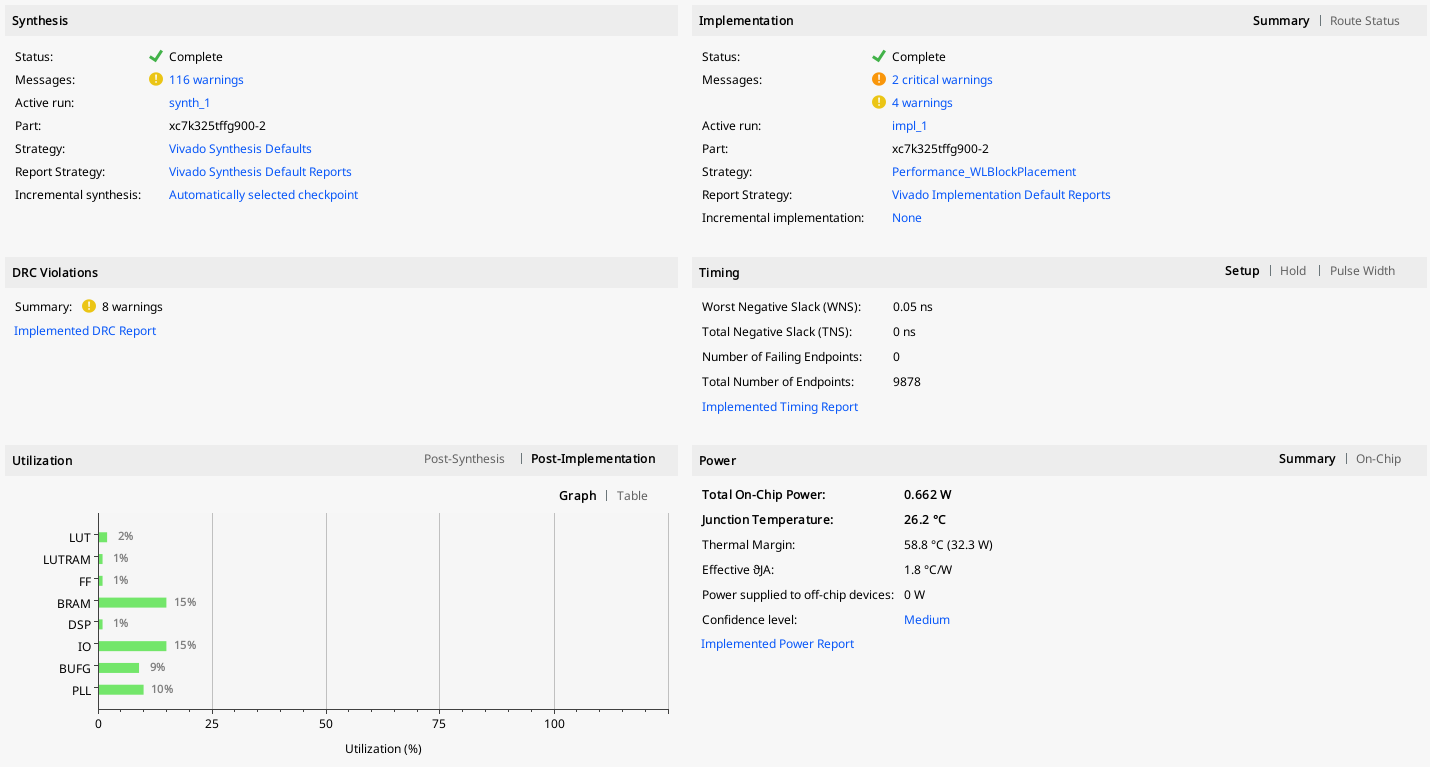
\includegraphics[width=0.96\linewidth]{快速预览-1.png}
  \caption{分赛区决赛版本实现与性能快速预览}
\end{figure}

该策略下，工程在 280 MHz 时钟约束下完成综合、实现和 bitstream 生成。布局布线后的最差时序裕量
WNS 为 +0.050 ns，无建立时间违例，说明设计满足 280 MHz 目标频率要求。结合数字孪生平台上五组程序的
实际运行结果，可以说明该版本不仅在工具实现层面通过高频约束，而且在板端运行中保持稳定。

\begin{figure}[H]
  \centering
  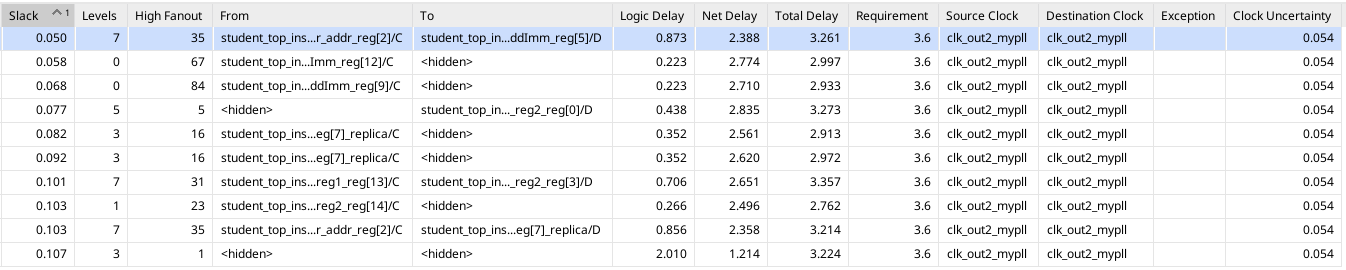
\includegraphics[width=0.96\linewidth]{快速预览-slack.png}
  \caption{280 MHz 时钟约束下 WNS 为 +0.050 ns}
\end{figure}

\subsection{RV32I指令支持情况说明}

本项目围绕 RV32I 基本整数指令集进行设计与验证。当前上板用例 src0、src1、src2 在实际运行过程中覆盖了算术逻辑运算、立即数运算、访存访问、条件分支以及 JAL/JALR 等典型执行路径；可以作为本项目支持 RV32I 指令执行能力的佐证。同时，后续的自动化测试流程将通过更全面的测试集验证处理器对 RV32I 的支持。


\newpage

\subsection{验证结果总结说明}

5 份测试用例均在 Vivado 2024.2 下无违例完成实现并成功生成比特流。

\begin{threelongtable}{@{}
  C{0.13\linewidth}
  C{0.29\linewidth}
  C{0.11\linewidth}
  C{0.16\linewidth}
  C{0.13\linewidth}@{}}
\caption{分赛区决赛上板测试结果}\\
\toprule
\textbf{测试用例} & \textbf{数字孪生平台状态} & \textbf{结果} & \textbf{性能测试用时} & \textbf{性能倍率}\footnotemark \\
\midrule
\endfirsthead
\toprule
\textbf{测试用例} & \textbf{数字孪生平台状态} & \textbf{结果} & \textbf{性能测试用时} & \textbf{性能倍率} \\
\midrule
\endhead
\bottomrule
\endlastfoot
src0 & 上板成功，界面运行正常 & 通过 & 7.101s & 4.00 \\
src1 & 上板成功，界面运行正常 & 通过 & 7.047s & 3.70 \\
src2 & 上板成功，界面运行正常 & 通过 & 9.233s & 4.00 \\
withoutMext & 上板成功，界面运行正常 & 通过 & 3.890s & --- \\
withMext & 上板成功，界面运行正常 & 通过 & 2.020s & 1.93\textsuperscript{*} \\
\end{threelongtable}
\footnotetext{src0、src1、src2 相对于赛题给出的 50 MHz 单周期参考设计；带 * 的 1.93 表示
withMext 相对于 withoutMext 的加速比。}

综上，分赛区决赛工程已经完成从设计实现、bitstream 生成到数字孪生上板验证的全流程闭环。
五组程序均在 280 MHz 下观察到正确运行结果，说明 CPU、FPGA 顶层封装、IROM/DRAM 初始化、
MMIO 输出路径及 RV32M 多周期乘除法单元工作正常。

\newpage

\part[仿真报告]{RISC-V CPU仿真报告}
\setcounter{section}{0}

\quickpreviewtitle

 \textbf{关键技术：}构建 Vivado Simulation 与 Verilator/C++ 双仿真平台；通过 DPI-C 实现 EBREAK 停机检测、
 LED/SEG 外设软件模拟和仿真串口输入，并接入 NEMU 作为差分测试参考模型。

 \textbf{测试覆盖：}完成 RV32I、RV32M 和 Zicsr 相关测试、小规模程序测试、官方 src0/src1/src2 性能测试、CoreMark、Dhrystone 
 以及 RT-Thread 基础命令测试；自动化流程已接入 GitHub Actions，支持提交后持续自动化集成测试。

\textbf{重要指标：}本次 CI 中官方三组性能测试的 CPI 分别为 1.4025、1.5131、1.3982，IPC 分别为
0.7130、0.6609、0.7152；280 MHz 估算时间分别为 7.10133 s、7.04752 s、9.23348 s。
CoreMark 为 308，CoreMark/MHz 为 1.10；Dhrystone 的 280 MHz 估算时间为 1.08042 s。

\textbf{作品亮点：}仿真系统不仅能判断程序是否运行正确，还能输出周期数、指令数、IPC、CPI、分支预测准确率
和 RAW 阻塞率等细粒度性能计数；同时支持 CSR、ecall、mret、csrrw、csrrs 等机制验证，为 RT-Thread 等更复杂软件负载运行提供基础。
且上板结果与仿真预测时间一致，说明仿真具备较高可信度。

\newpage

\section{仿真平台介绍}

\subsection{仿真工具}

本项目中使用的仿真工具分为两类：一类为 Vivado Simulation 自带的仿真工具，用于进行包含数码管、LED、BRAM 等板级外设后的板级行为正确性仿真和时序后仿。另一类为基于 Verilator 和 C/C++ 搭建的高性能行为仿真平台，便于快速仿真、实现自定义需求功能。

\subsection{测试环境说明}

\subsubsection{Vivado 仿真测试平台}

仿真环境 Vivado 2024.2，Windows 本地工程，使用 Run Behavioral Simulation 观察波形，检查是否向数码管等外设写入预期正确值。

\begin{figure}[H]
  \centering
  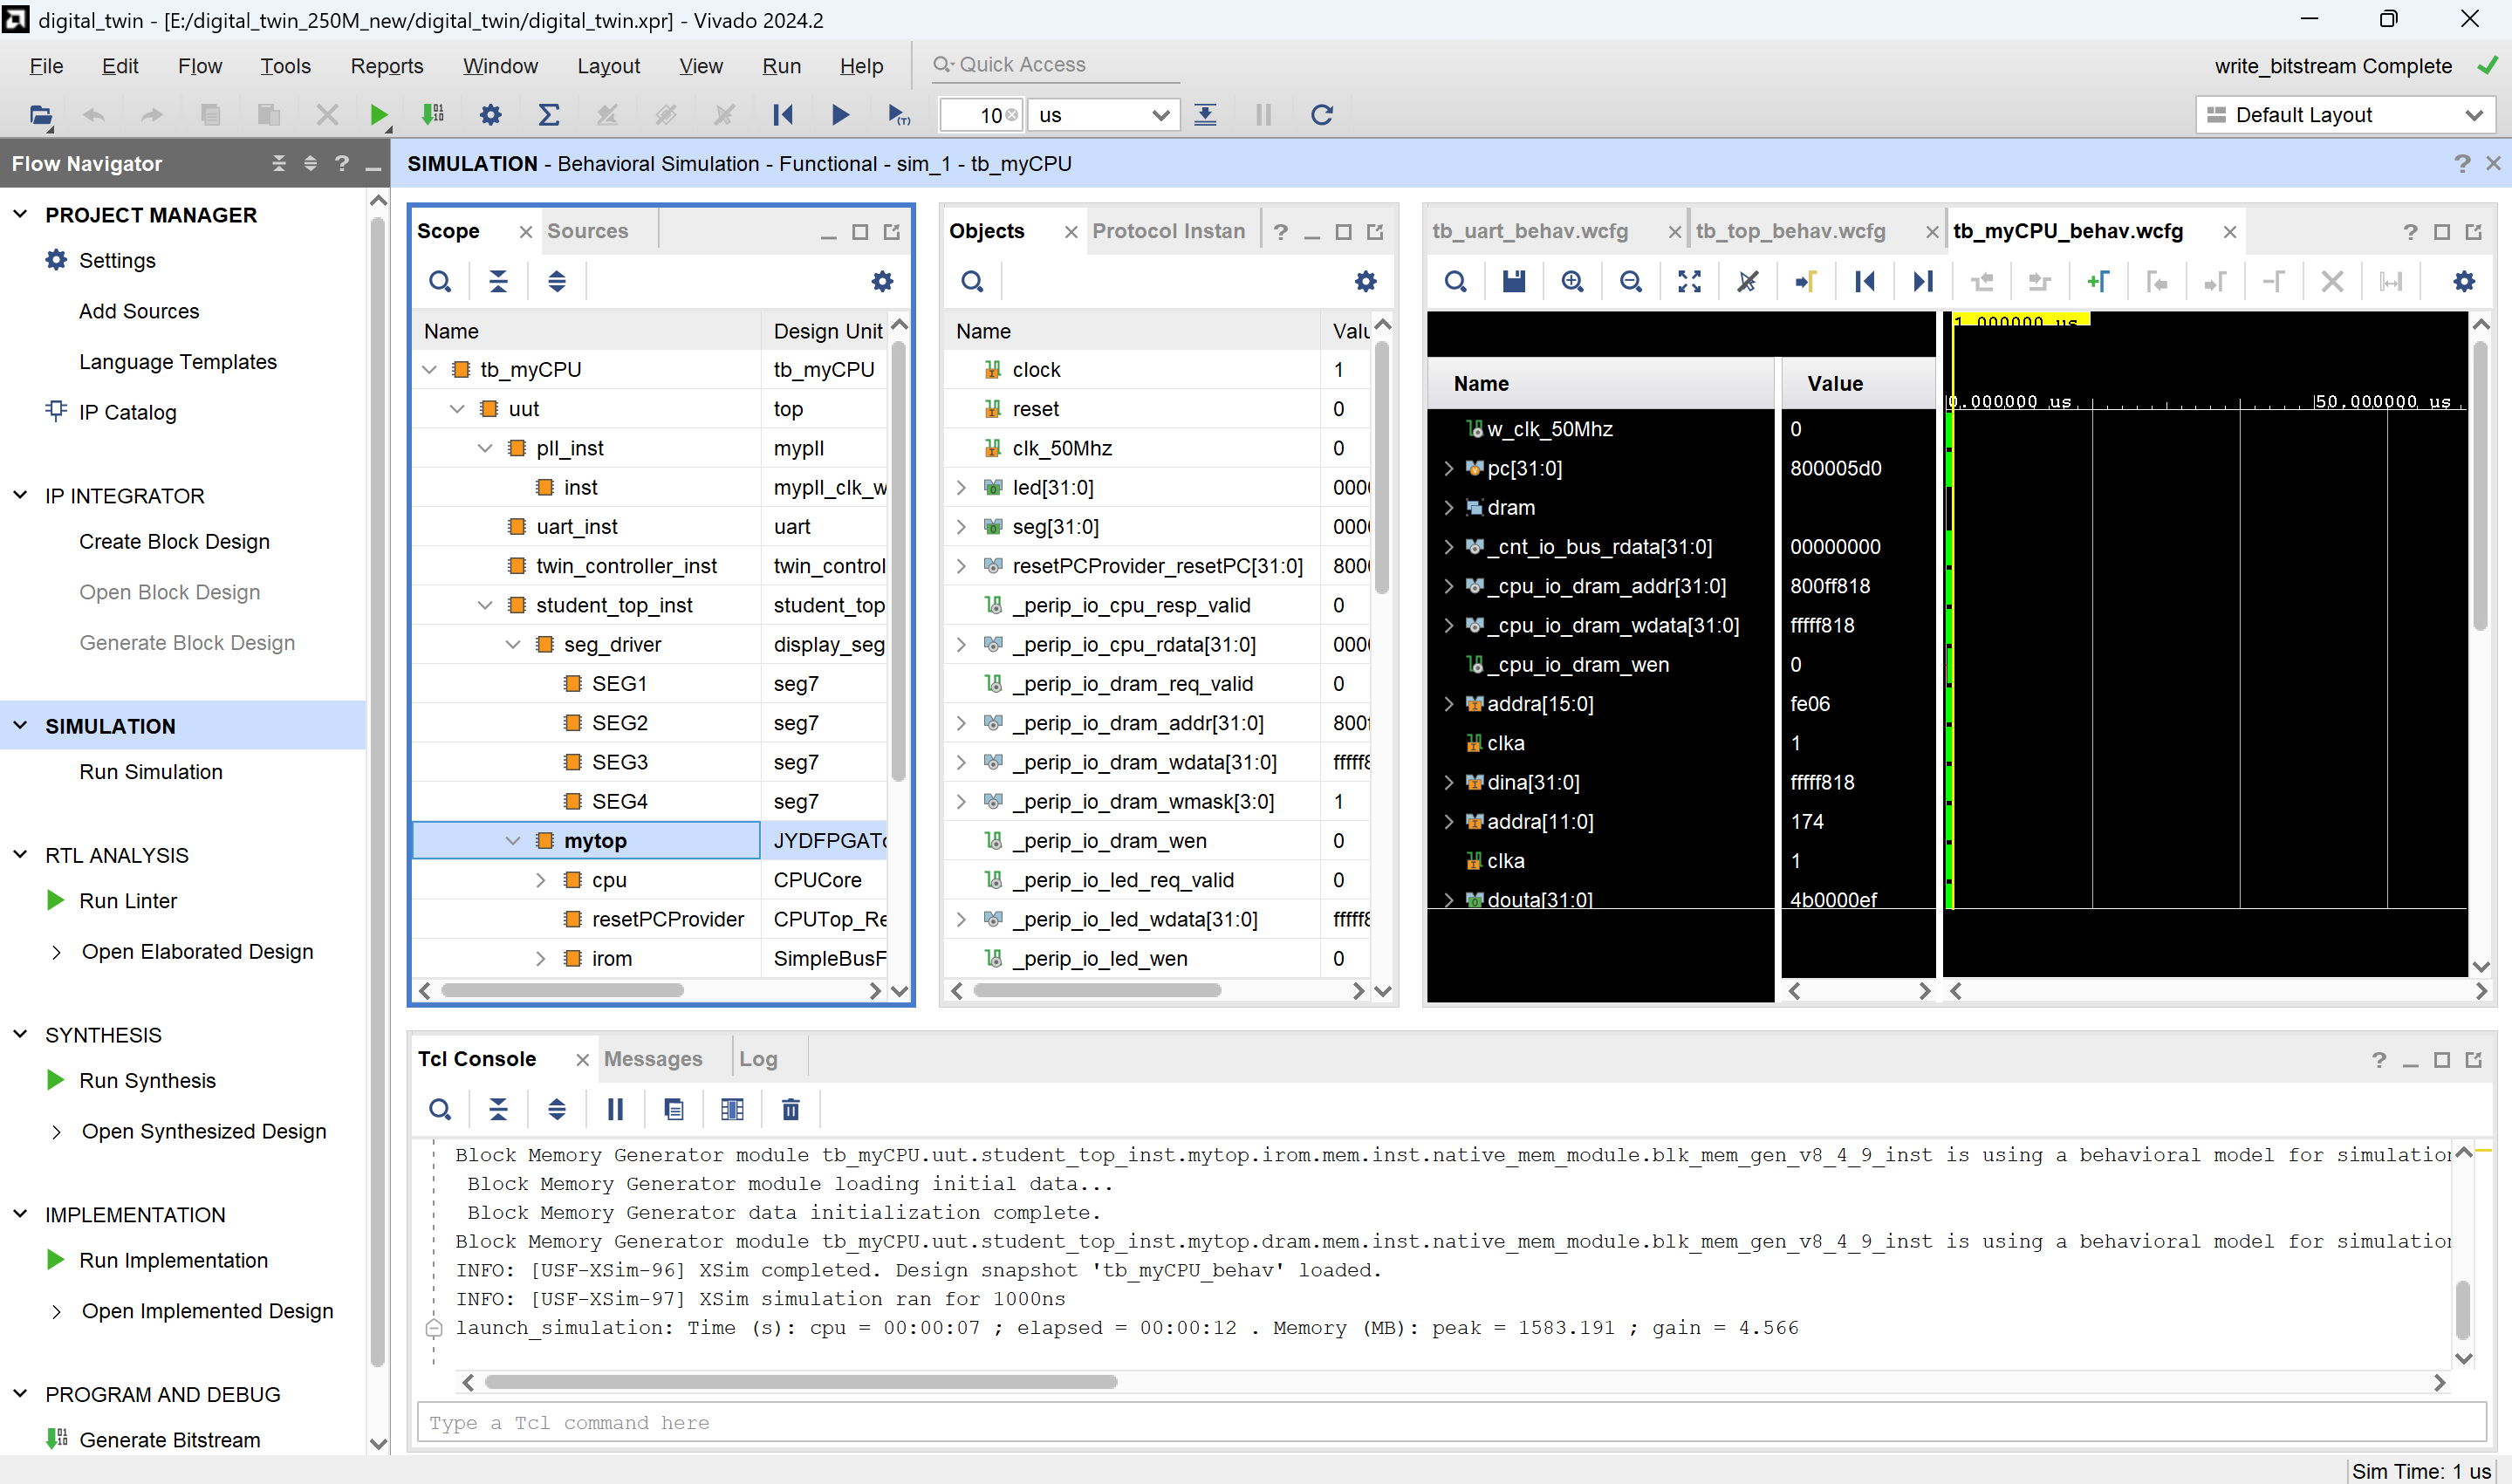
\includegraphics[width=\linewidth]{image8.png}
  \caption{Vivado 仿真工程界面}
\end{figure}

\subsubsection{Verilator 仿真测试平台}

实现了性能统计、差分测试、行为踪迹、流水线日志、接入 GitHub Actions 自动化集成测试。测试仿真日志中的 Perf Counters Report 统计了周期数、指令数、IPC、CPI、分支预测准确率和 RAW stall 等性能指标。

项目 CPU 通过直接编程接口（DPI-C）方法实现了 EBREAK 的仿真时支持，通过为测试程序提供基础运行库使其停机（halt）后执行 EBREAK，触发仿真程序检查 a0 寄存器作为 main 函数返回值是否为 0 来判定测试程序是否正确运行。并使用了软件 RISC-V 模拟器\footnote{参考了\href{https://ysyx.oscc.cc/docs/}{一生一芯项目}对 CPU 测试的资料，软件模拟器 NEMU 在其讲义指导下独立实现完成。}，作为差分测试的参考执行。

同时使用 DPI-C 方法在软件层面模拟了竞业达板卡的 LED 和 SEG 外设，使得可以运行官方 coe 文件，拥有相对一致的外设行为。

并参考一生一芯项目 B 线 CI 测试\footnote{因 B 阶段 CI 测试仍处于内测阶段，根据相关要求，暂不便提供参考链接。}，
基于 GitHub Actions 搭建了自动化正确性测试、性能测试和 Vivado 执行流程。本次分赛区决赛版本
对应的 CI 记录为 \href{https://github.com/HanPiM/jyd/actions/runs/29162587063}{Actions run 29162587063}，
其中用户提供的 \texttt{withMext-v2} 任务记录为
\href{https://github.com/HanPiM/jyd/actions/runs/29162587063/job/86570180985}{job 86570180985}；
被测提交为 \texttt{585ebc2b7f41ea65fb4c6536f9a6747171495258}。

\begin{figure}[H]
  \centering
  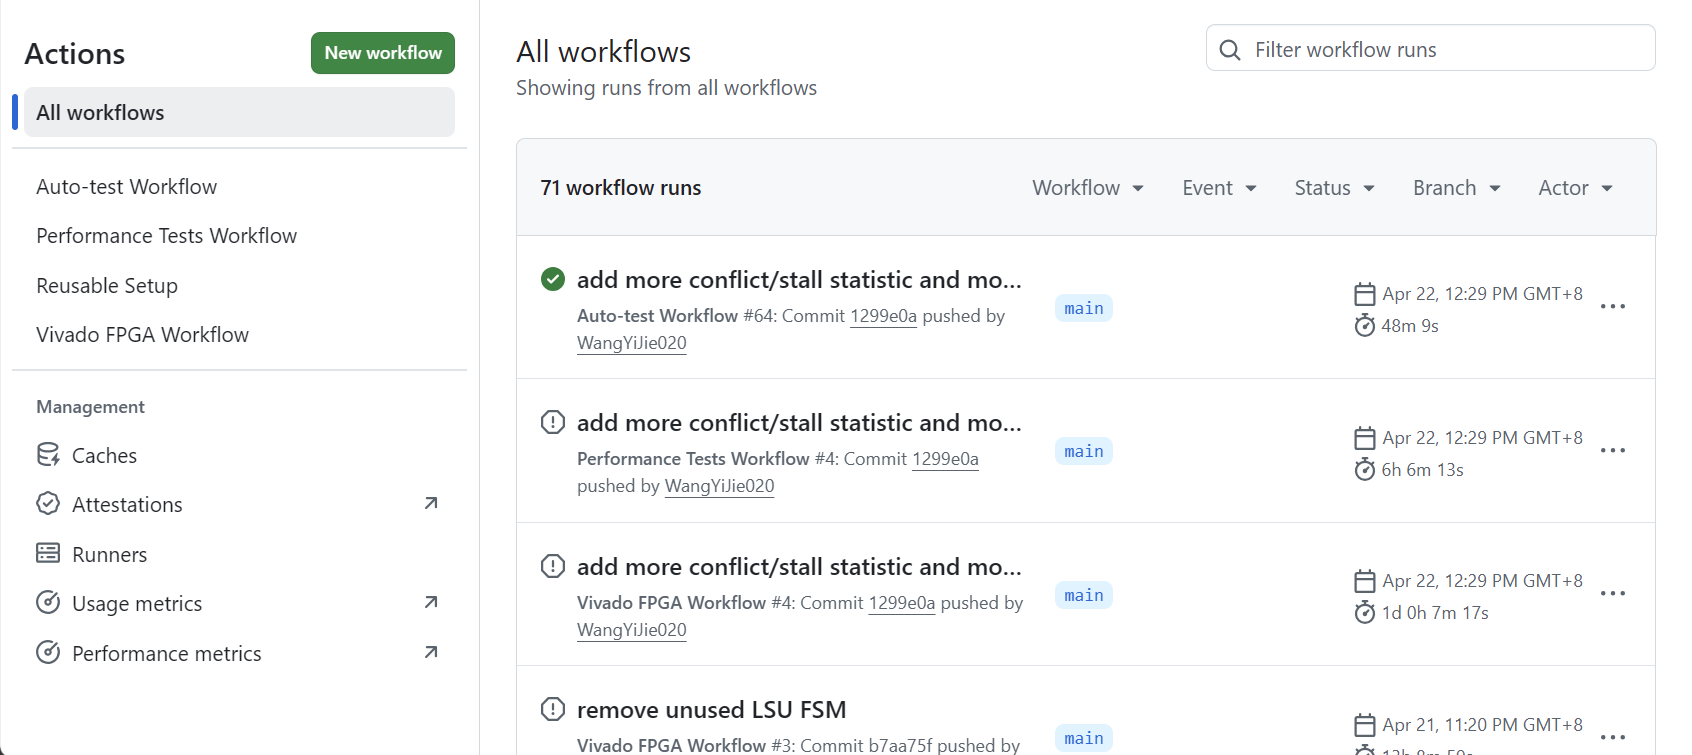
\includegraphics[width=\linewidth]{image9.png}
  \caption{GitHub Actions 界面}
\end{figure}

每次提交新代码后会自动触发系列测试运行，具体测试流程：对于 C 代码测试程序，使用 riscv64-linux-gnu 工具链编译成二进制文件、使用 riscv64-linux-gnu-objcopy 提取 .text 段和 .data 段作为 IROM 和 DRAM 初始化数据、执行仿真直到 EBREAK、检查正确性；对于 coe 文件，使用脚本转换为二进制文件后同上流程进行仿真。

\section{RV32I CPU 测试}

\subsection{RV32I指令集测试}

针对 RV32I 指令集的测试，采用了单指令单元测试和小规模程序测试的方法验证。测试项目选用了南京大学相关实验项目提供的基于裸机运行环境的开源 RISC-V 测试集。

\begin{figure}[H]
  \centering
  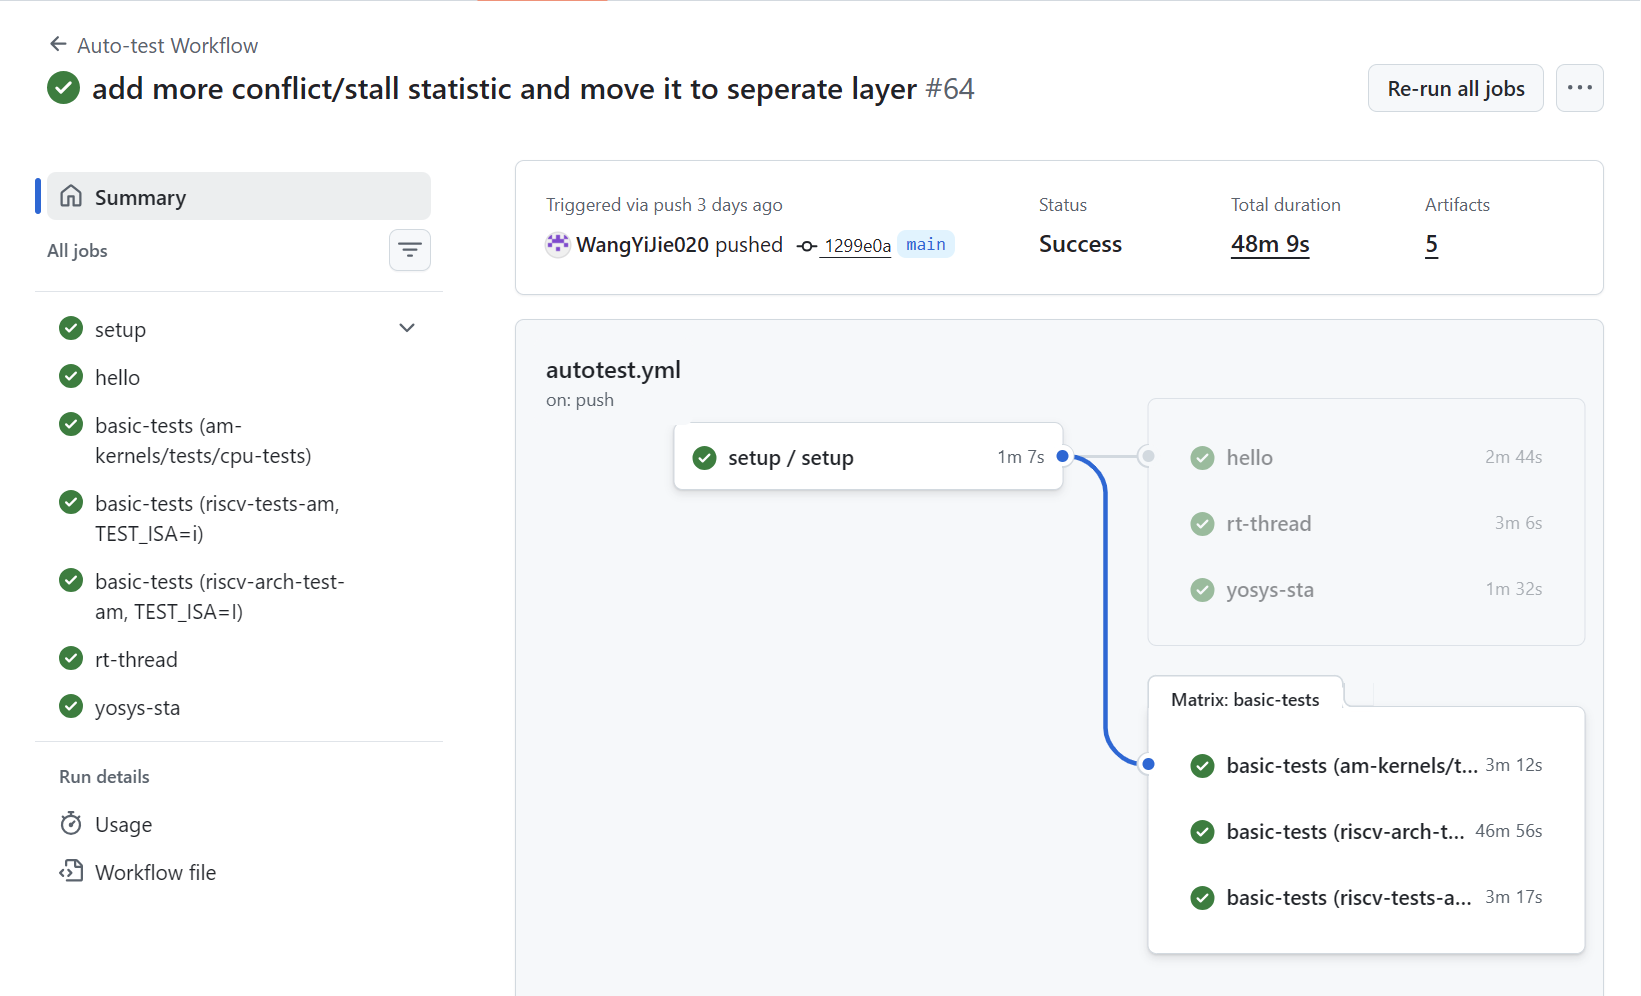
\includegraphics[width=0.92\linewidth]{image10.png}
  \caption{正确性测试自动化流程界面}
\end{figure}

项目提交时的版本对应测试记录为
\href{https://github.com/HanPiM/jyd/actions/runs/29162587063}{HanPiM/jyd@585ebc2b}。

对于单元测试，项目选用了下列测试集测试每个指令以及其边界情况，从指令级别对 CPU 进行了较为完备的基础测试。

\begin{itemize}
	\item \href{https://github.com/NJU-ProjectN/riscv-tests-am}{NJU-ProjectN/riscv-tests-am}：移植到 AM \footnote{南京大学计算机实验中对裸机环境的一层抽象环境} 的 \href{https://github.com/riscv-software-src/riscv-tests}{riscv-tests} 测试集。
  \item \href{https://github.com/NJU-ProjectN/riscv-arch-test-am}{NJU-ProjectN/riscv-arch-test-am}：移植到 AM 的 \href{https://github.com/riscv/riscv-arch-test}{riscv-arch-test} 测试集。
  \item 对于小规模程序测试，使用了 \href{https://github.com/NJU-ProjectN/am-kernels}{NJU-ProjectN/am-kernels: AbstractMachine kernels}，其中 tests/cpu-tests 提供了简易程序级测试负载。
\end{itemize}

\subsection{RV32I CPU性能测试}

性能测试选用了官方给出的 src0、src1、src2 三个性能测试，以及额外的由 NJU-ProjectN/am-kernels 移植提供的 coremark、dhrystone 跑分测试项。因为仿真的时序信息不准确，Counter 计时器连接的时钟和 CPU 时钟相同，预测的运行时间通过 Cycle 数另外计算。

\begin{figure}[H]
  \centering
  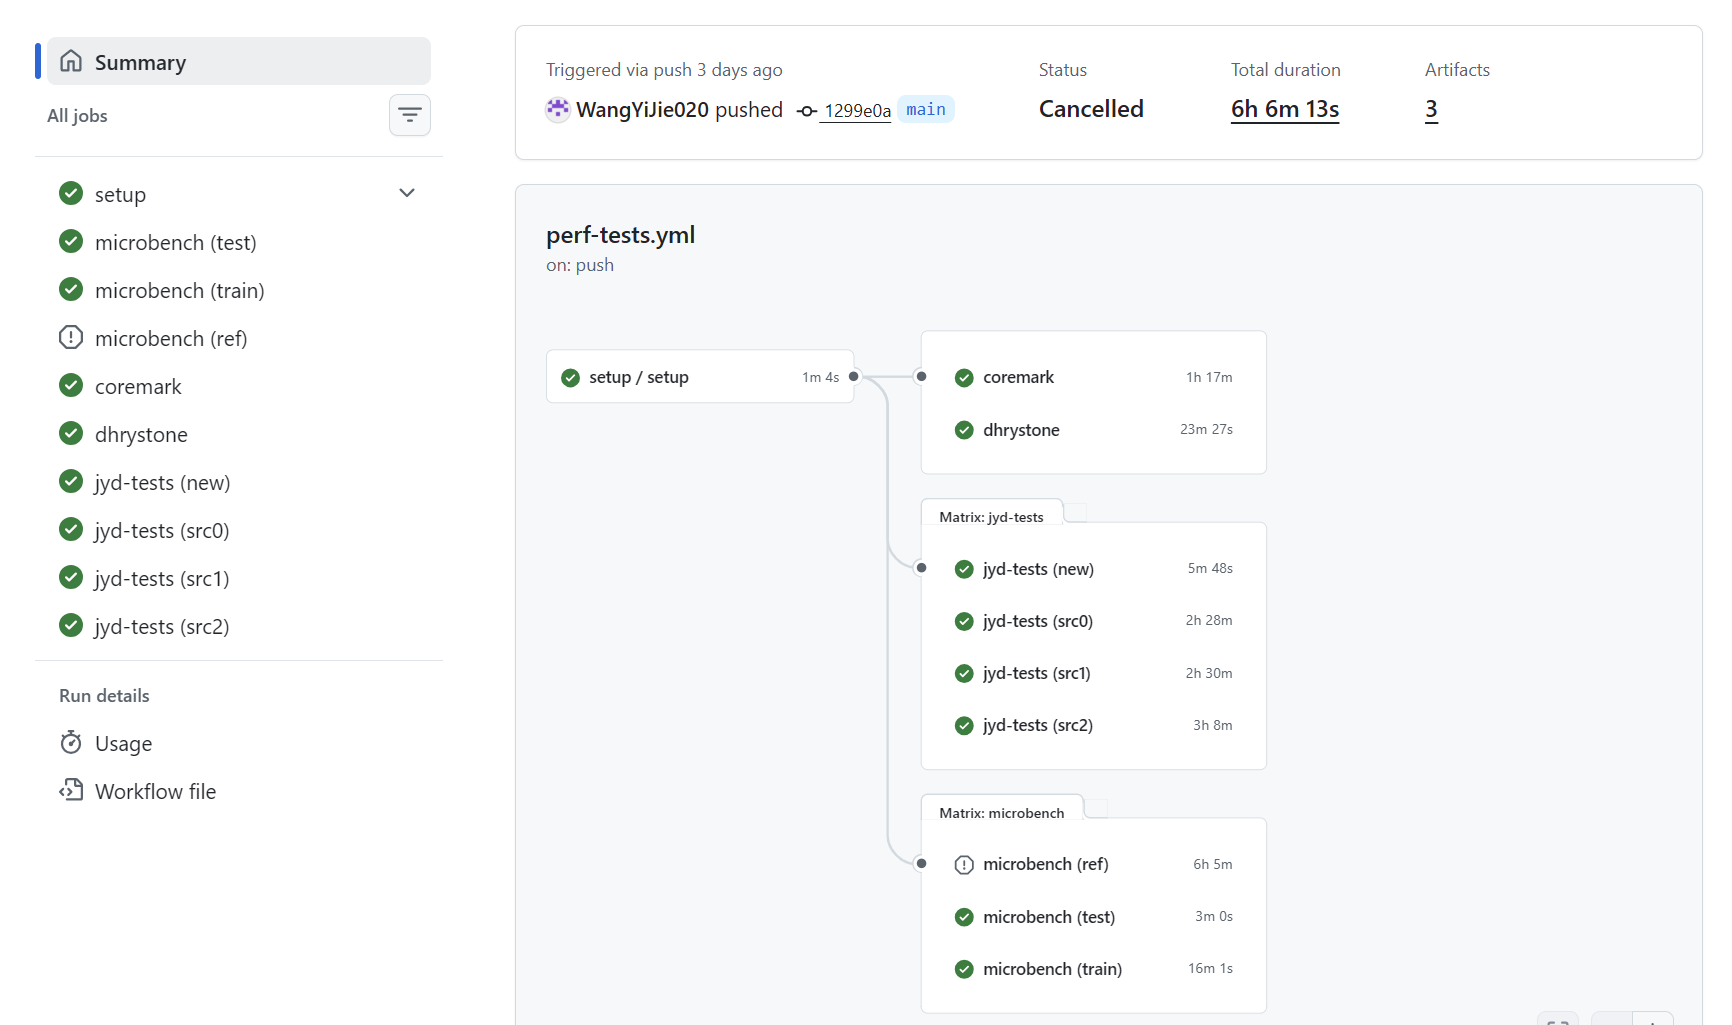
\includegraphics[width=\linewidth]{image11.png}
  \caption{性能测试自动化流程界面}
\end{figure}

\subsection{RV32I CPU 其他测试}

CPU 支持了部分 CSR 寄存器：mcycle(h)、mstatus、mepc、mtvec、marchid、mvendorid，支持了 ecall、mret、csrrw、csrrs 指令。并基于南京大学计算机实验教学版本 RT-Thread 分支 \href{https://github.com/NJU-ProjectN/rt-thread-am}{NJU-ProjectN/rt-thread-am}（不能直接运行，仅将依赖库替换为了 AM 裸机环境），参考南京大学计算机实验的讲义\footnote{\href{https://ysyx.oscc.cc/docs/ics-pa/4.1.html\#rt-thread-\%E9\%80\%89\%E5\%81\%9A}{RT-Thread 选做讲义}。}，独立完成了软件上 BSP 部分依靠 CSR 进行上下文切换的实现，从而能够支持 RT-Thread 的运行。同时为方便测试，为 CPU 添加了仿真层面的串口可以进行输入。

% \begin{figure}[H]
%   \centering
%   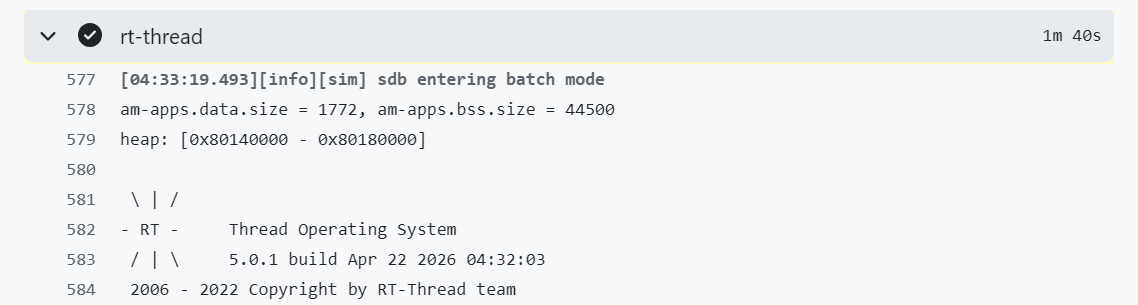
\includegraphics[width=0.82\linewidth]{image12.png}
%   \caption{RT-Thread 启动输出}
% \end{figure}

自动化测试流程为使用脚本\footnote{参考了一生一芯项目 B 阶段 CI 测试的脚本。}启动仿真后向标准输入流写入测试命令，监测输出是否出现预期结果。


\section{仿真结果}

\subsection{RV32I指令集测试结果}

\subsubsection{RV32I基本指令测试结果}

\begin{figure}[H]
  \centering
  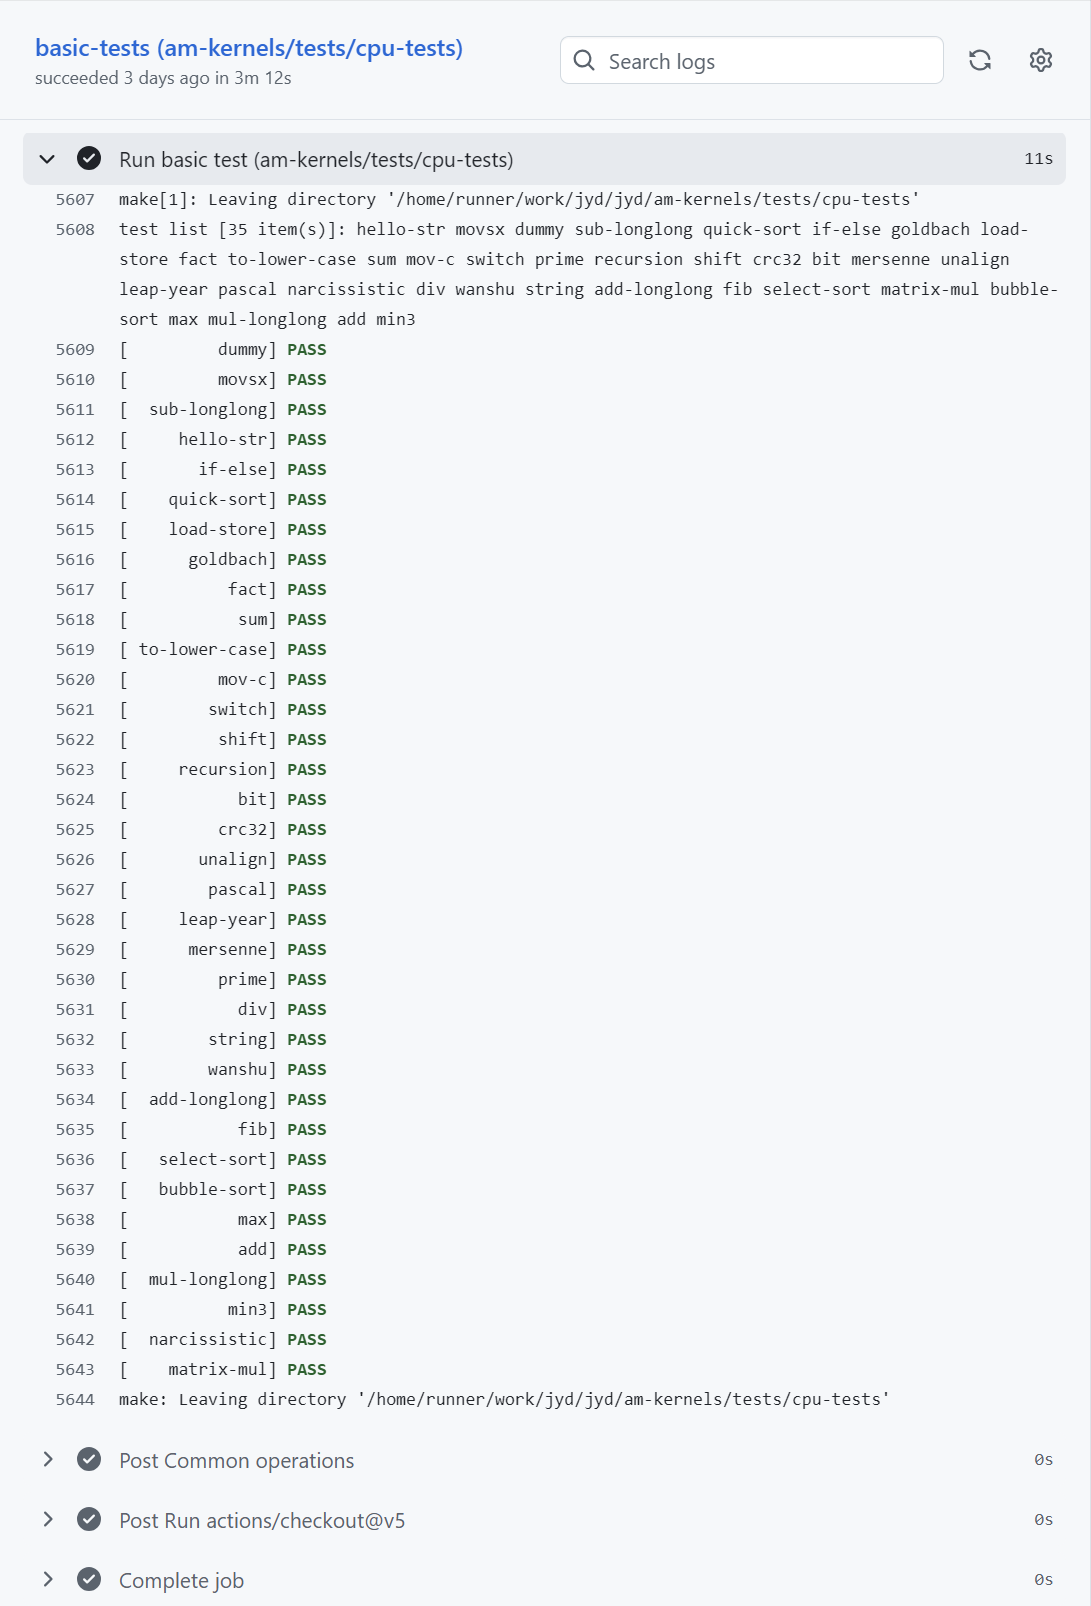
\includegraphics[height=0.64\textheight,trim=0 0 669bp 0,clip]{image13.png}%
  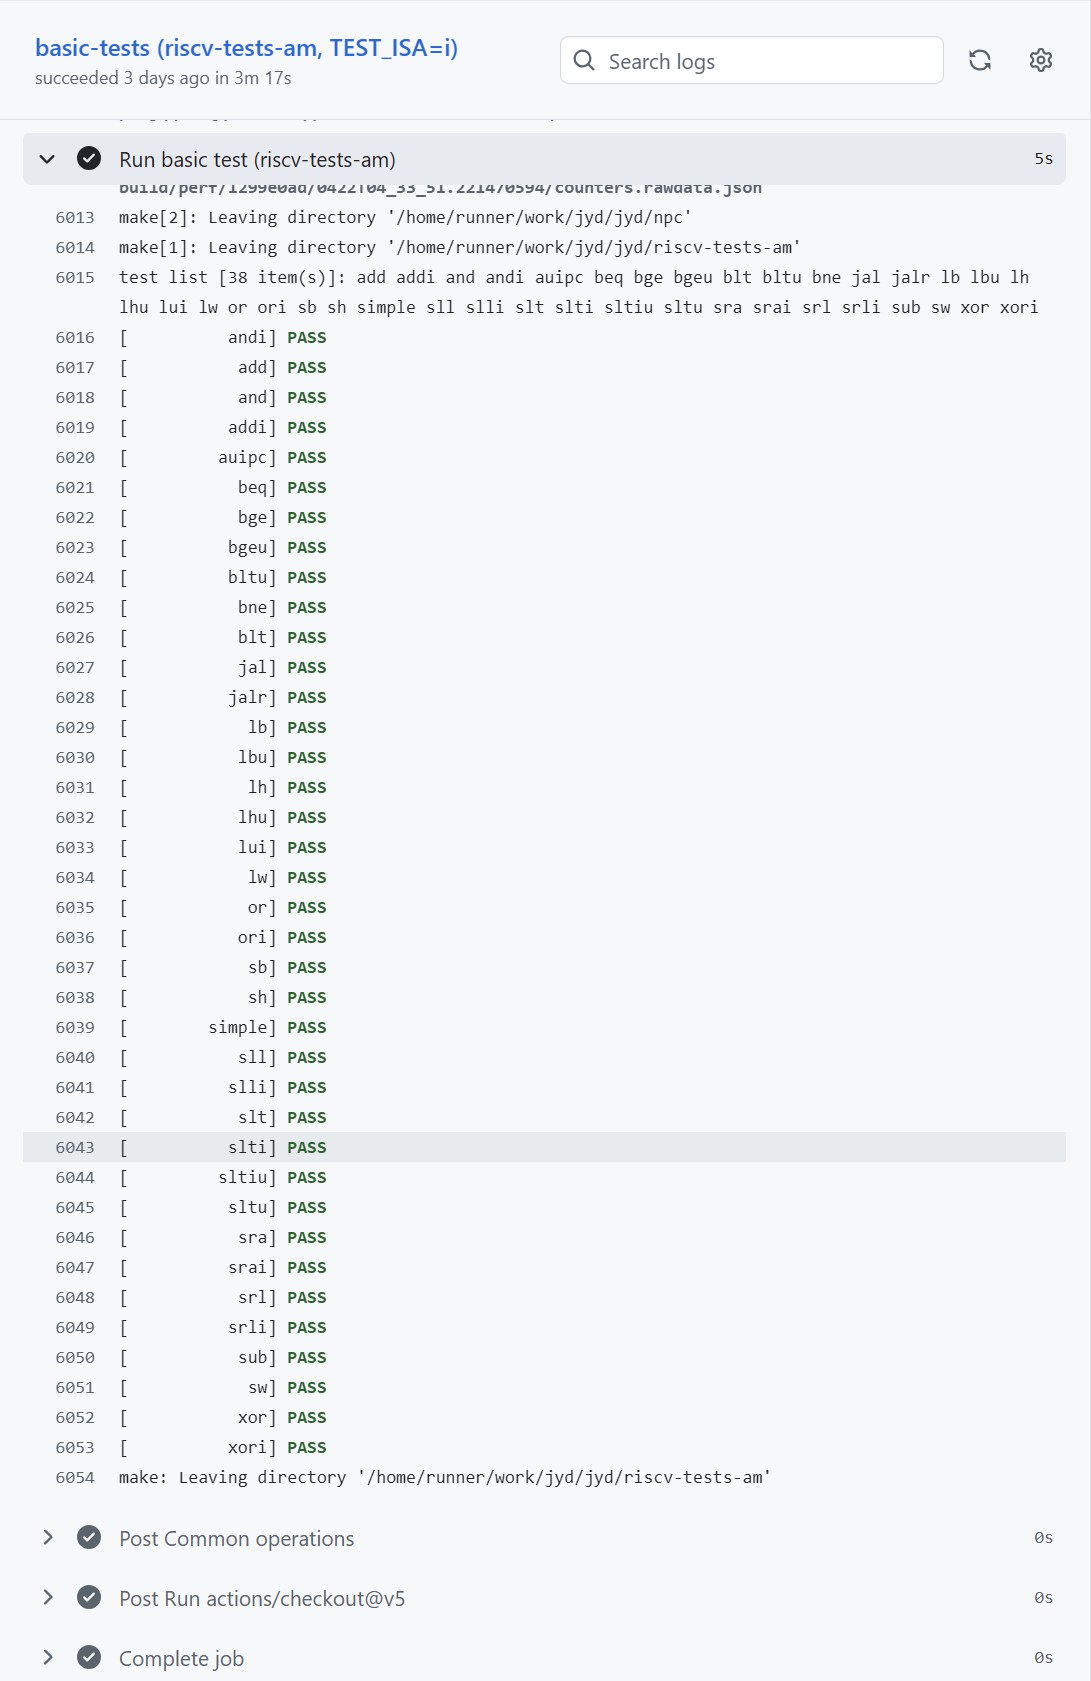
\includegraphics[height=0.64\textheight,trim=0 0 644bp 0,clip]{image14.png}%
  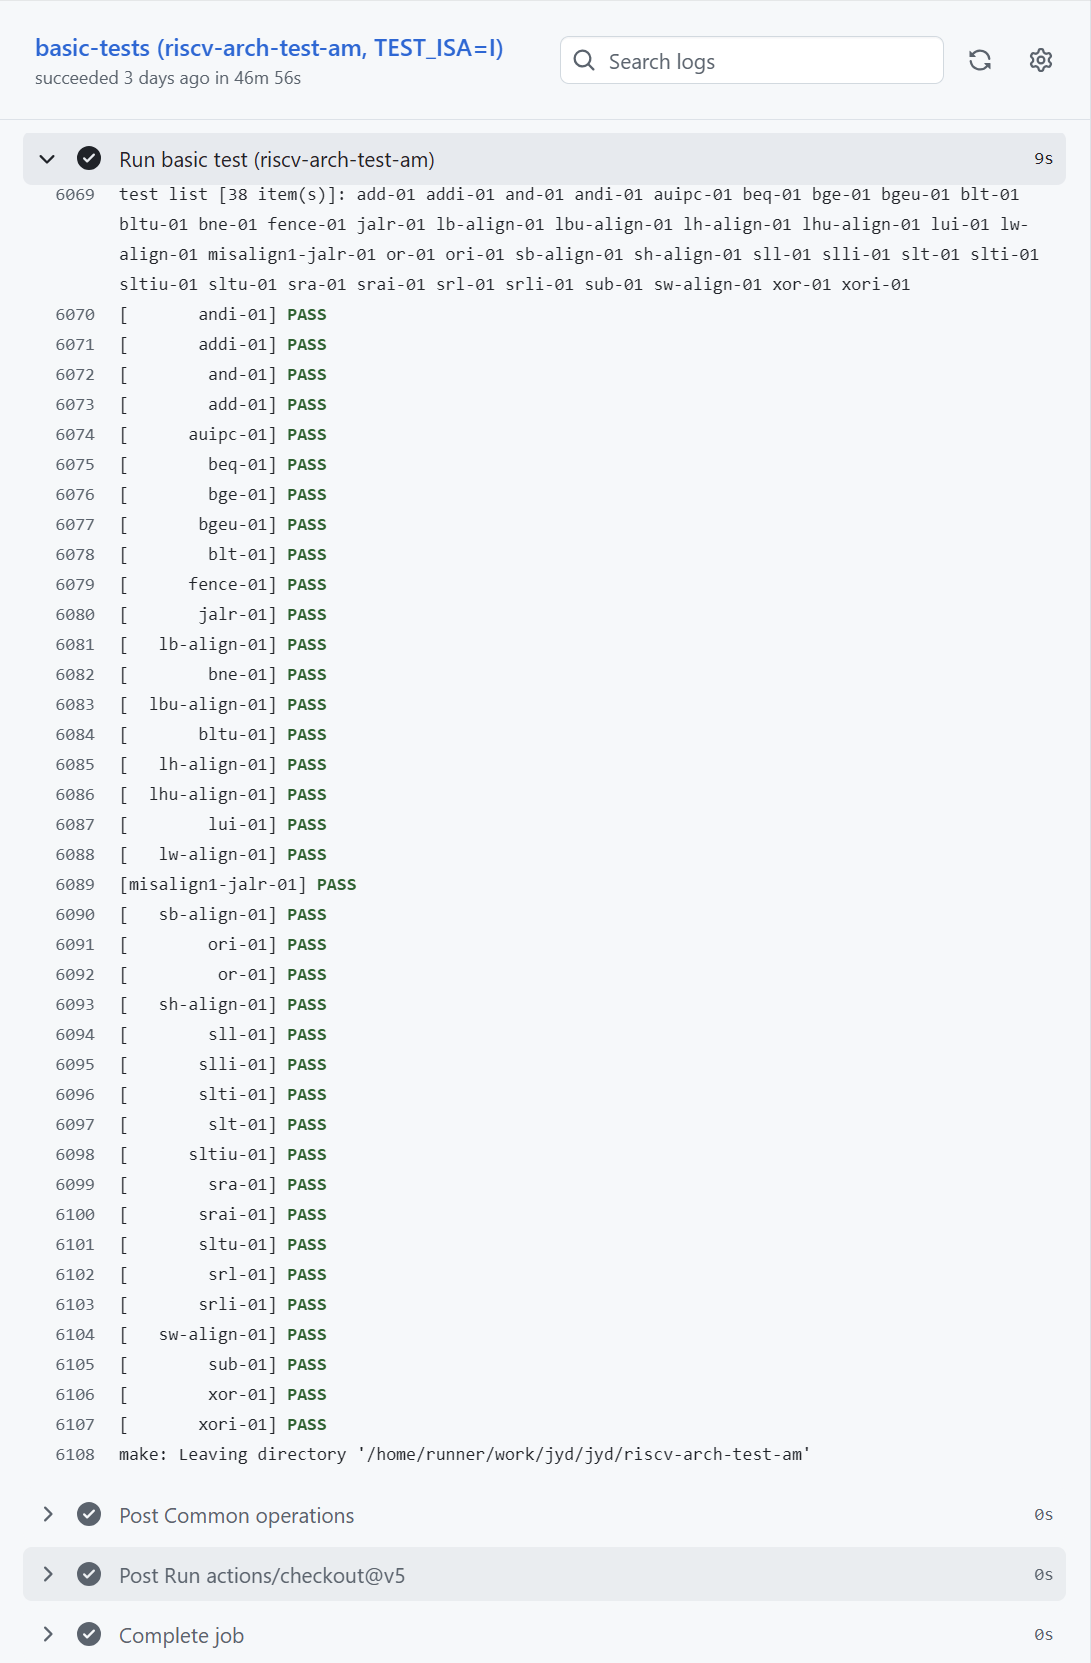
\includegraphics[height=0.64\textheight,trim=0 0 654bp 0,clip]{image15.png}
  \caption{RV32I 基本指令测试结果截图}
\end{figure}

从图片可以看出所有测试均成功通过，表明 CPU 支持 RV32I 且能够正确处理边界样例。

\subsection{RV32I CPU性能测试结果}

\subsubsection{src0性能测试用例}

\begin{figure}[H]
  \centering
  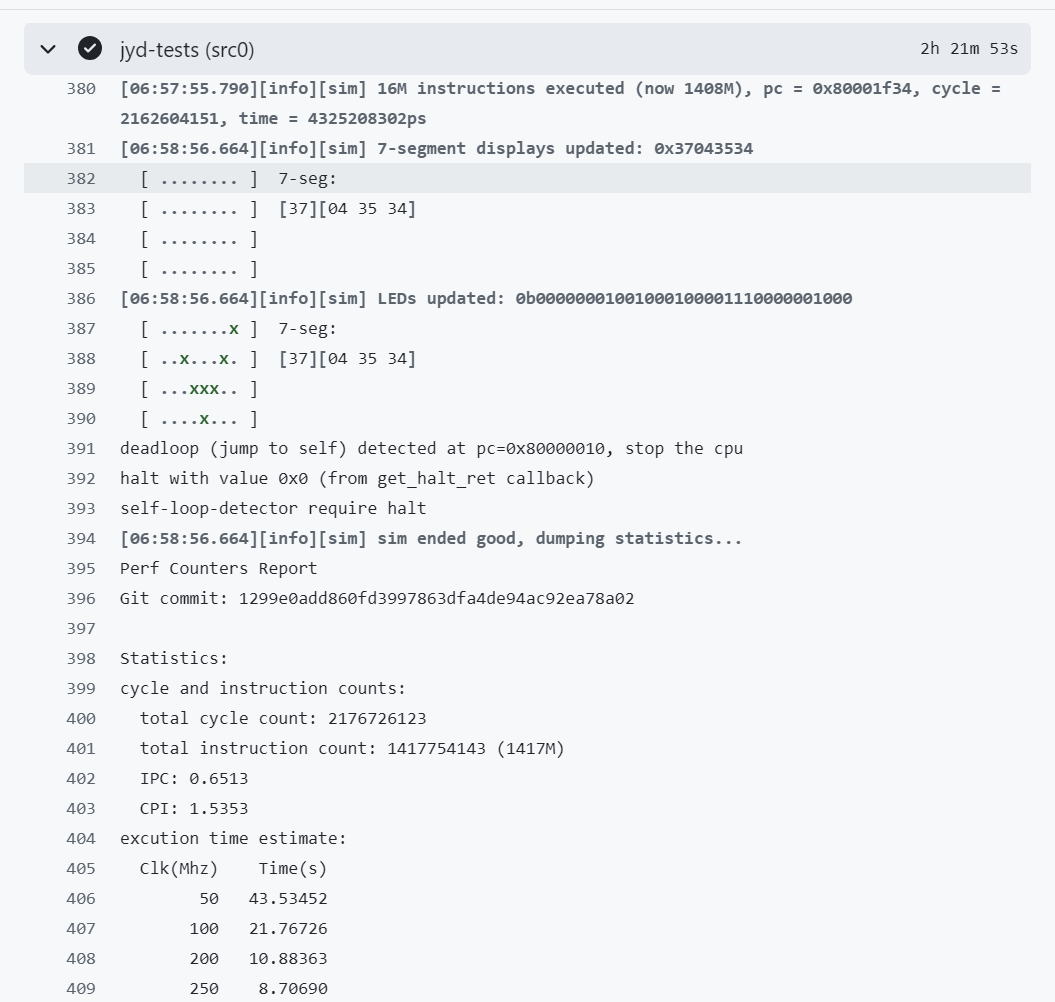
\includegraphics[width=0.84\linewidth,trim=0 365bp 0 0,clip]{image16.png}
  \caption{src0 仿真日志与性能统计结果}
\end{figure}

测试程序 src0 成功在仿真末尾观测到数码管和 LED 更新为预期结果，表明 37 条指令测试和性能测试均通过。
程序最终进入 halt 死循环并被仿真正确识别。本次 CI 统计总周期数为 1,988,372,516，按 280 MHz
计算，预测运行时间为 $1,988,372,516/(280\times10^6)=7.10133$ s，与上板显示的 7.101 s 一致。

仿真性能计数器显示\footnote{性能统计截图暂沿用初赛版并裁去下方旧 CPI 数据；决赛版原始数据以本次 CI 日志为准。}
总周期数为 1988M，总动态指令数为 1417M，IPC 为 0.7130，CPI 为 1.4025。

\begin{figure}[H]
  \centering
  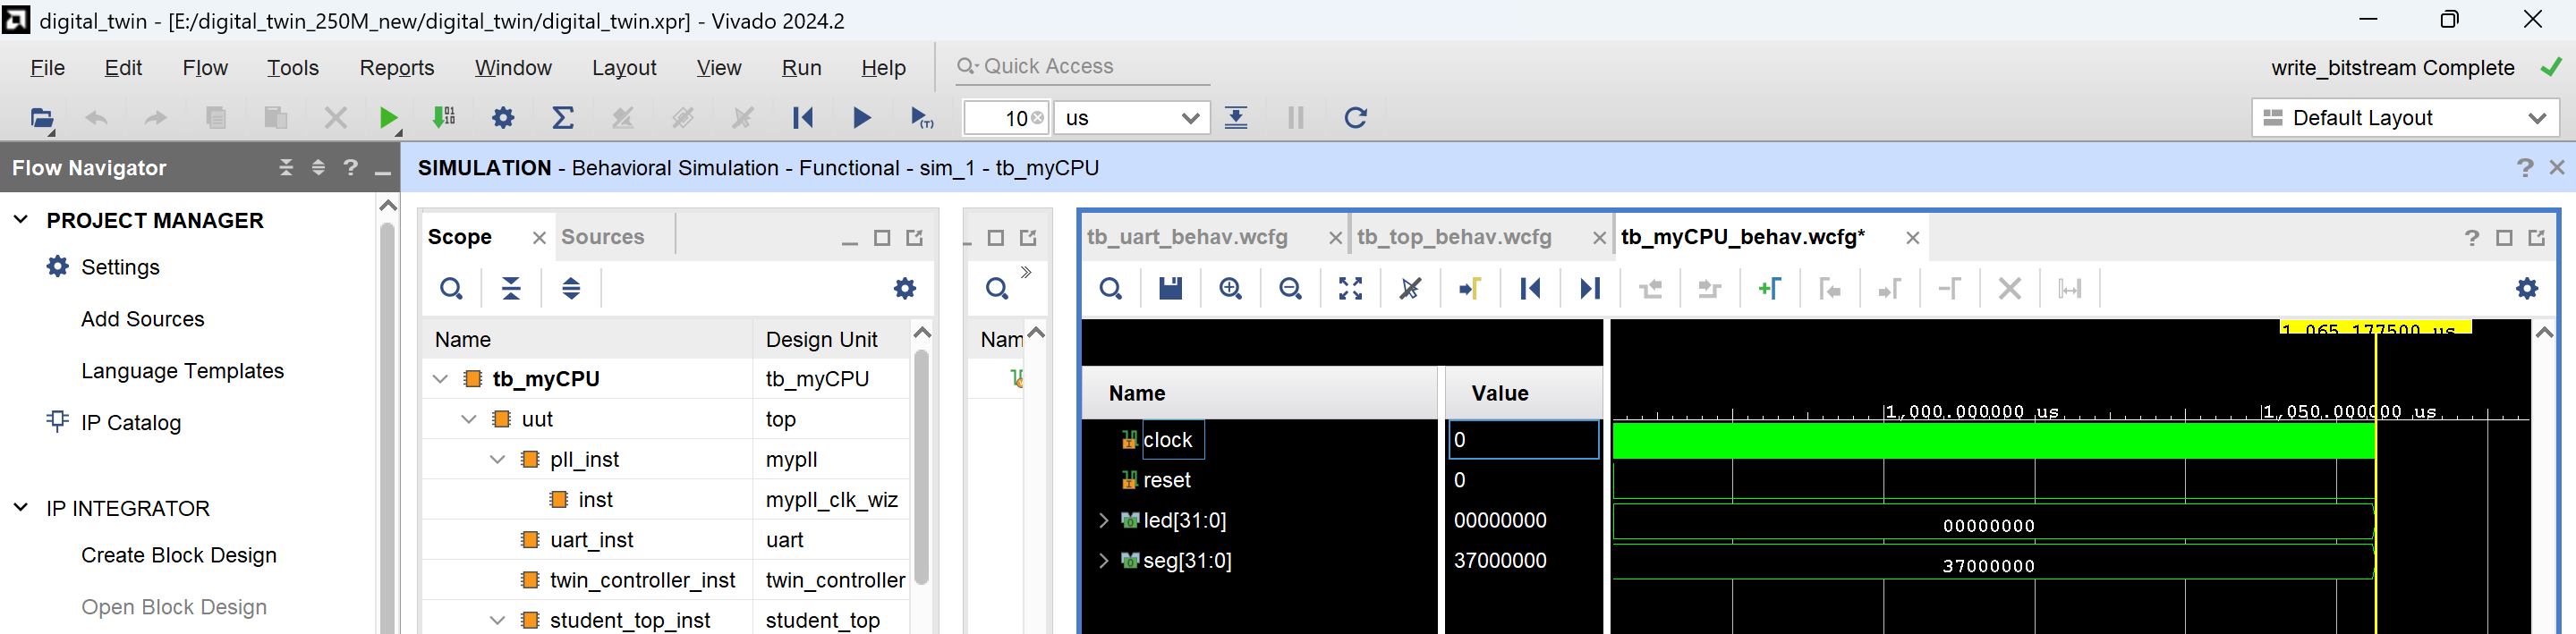
\includegraphics[width=\linewidth]{image17.png}
  \caption{src0 仿真波形结果}
\end{figure}

因 Vivado 仿真速度较慢，只仿真到数码管显示 37000000 证明 37 条指令测试正确通过，未完整运行至性能测试结束。

\subsubsection{src1性能测试用例}

\begin{figure}[H]
  \centering
  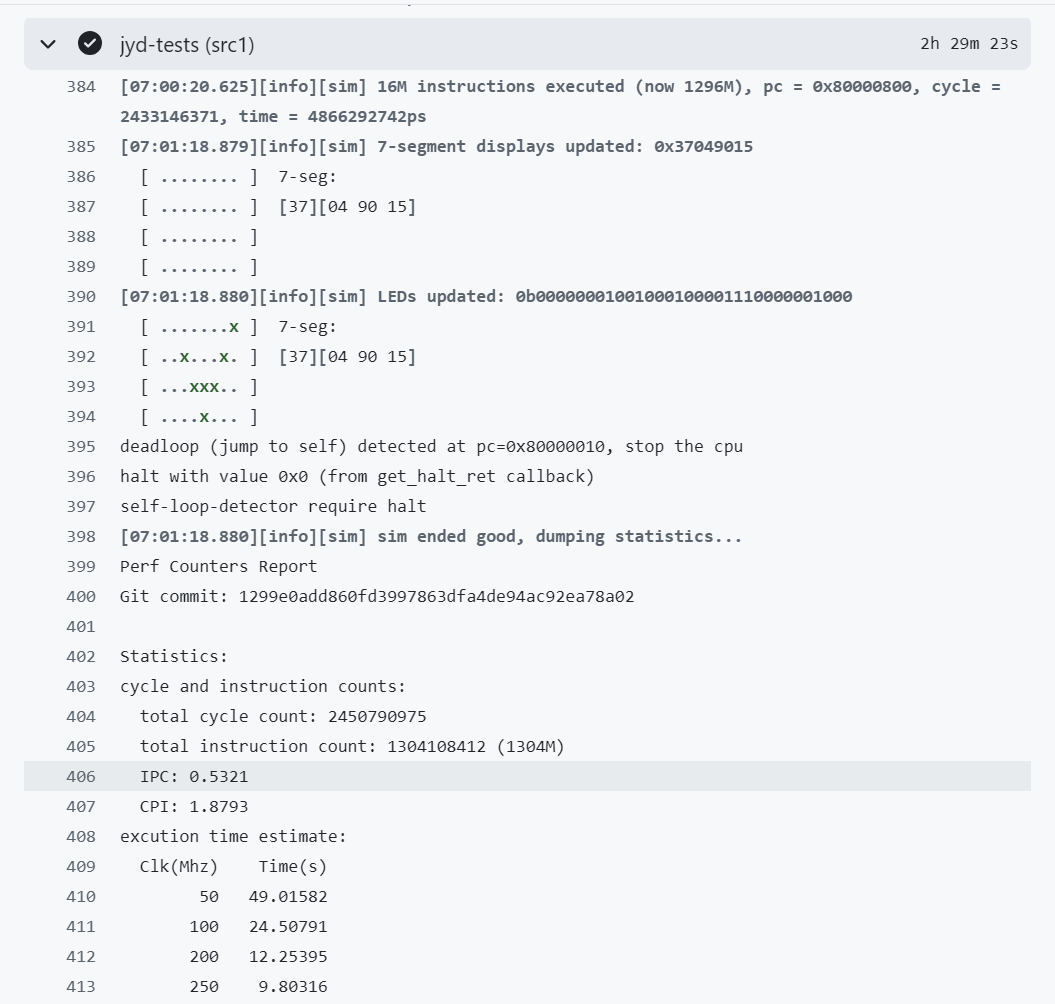
\includegraphics[width=0.82\linewidth,trim=0 350bp 0 0,clip]{image18.png}
  \caption{src1 仿真日志与性能统计结果}
\end{figure}

37 条指令测试通过。总周期数为 1,973,306,668，280 MHz 预测运行时间为 7.04752 s，
与实际上板测试结果 7.047 s 一致。

仿真性能计数器显示总周期数为 1973M，总动态指令数为 1304M，IPC 为 0.6609，CPI 为 1.5131。

\begin{figure}[H]
  \centering
  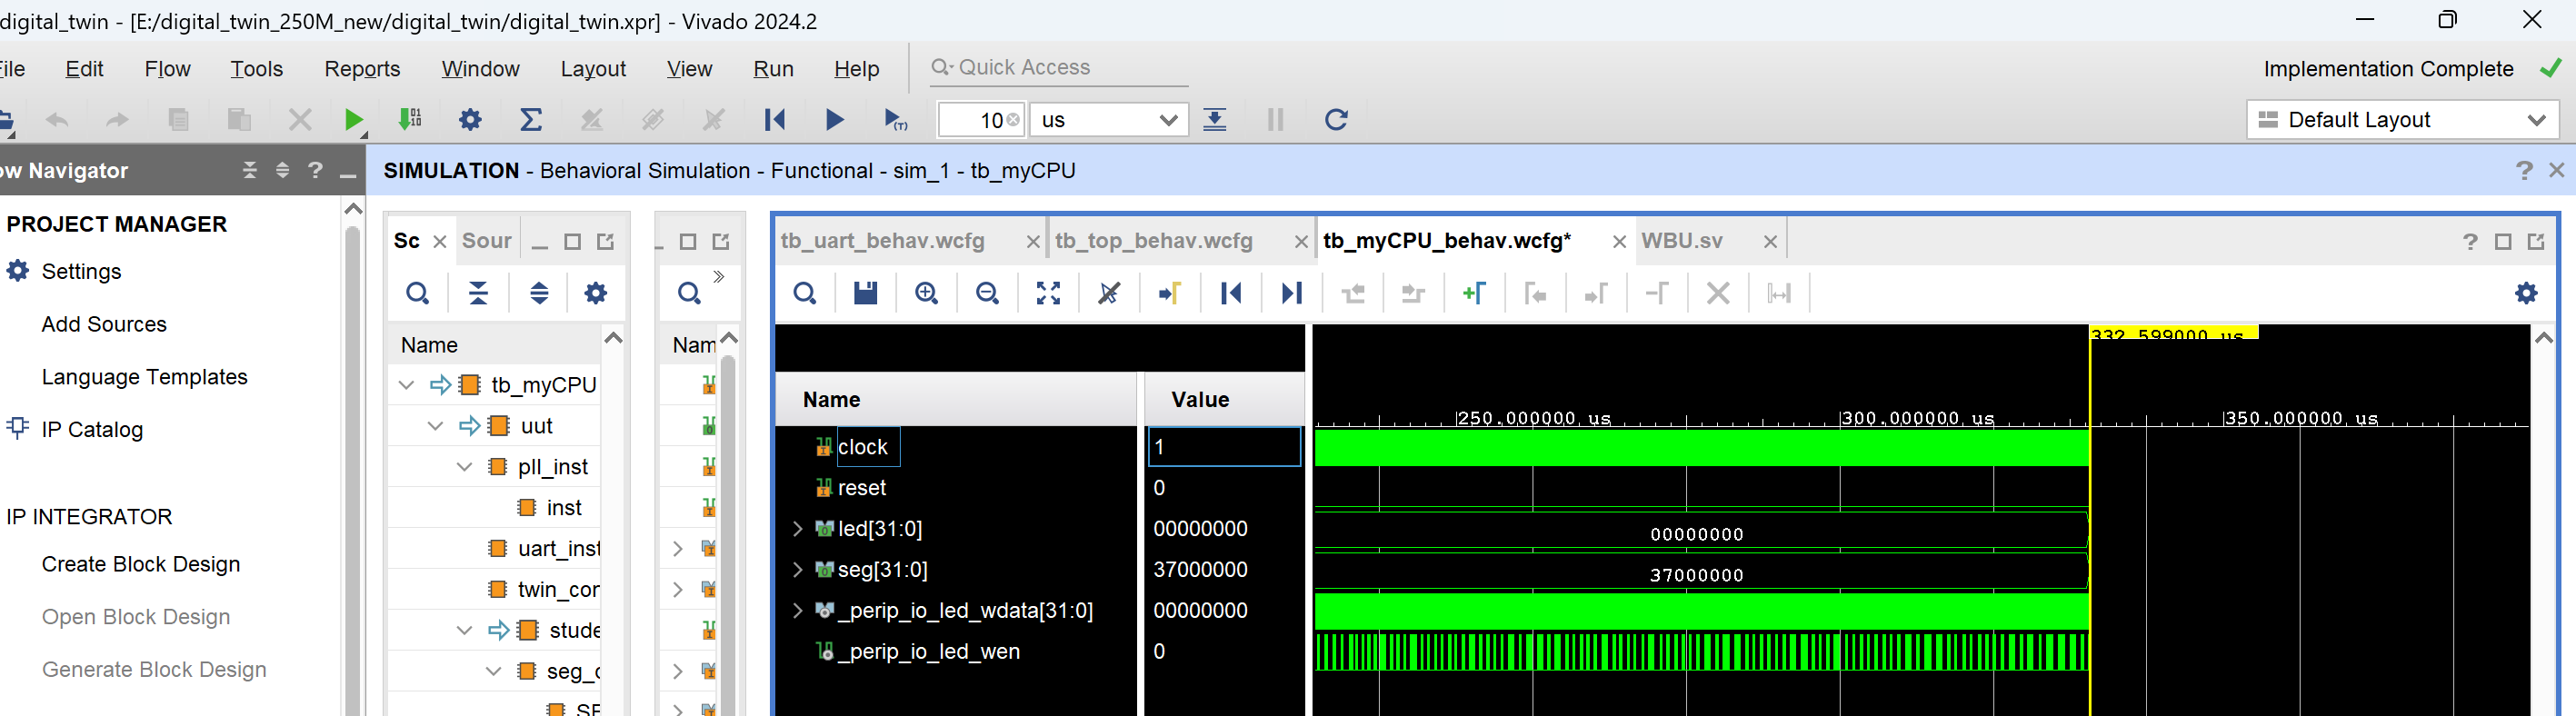
\includegraphics[width=\linewidth]{image19.png}
  \caption{src1 仿真波形结果}
\end{figure}

由图可知，数码管显示 37000000 证明 37 条指令测试正确通过。

\subsubsection{src2性能测试用例}

\begin{figure}[H]
  \centering
  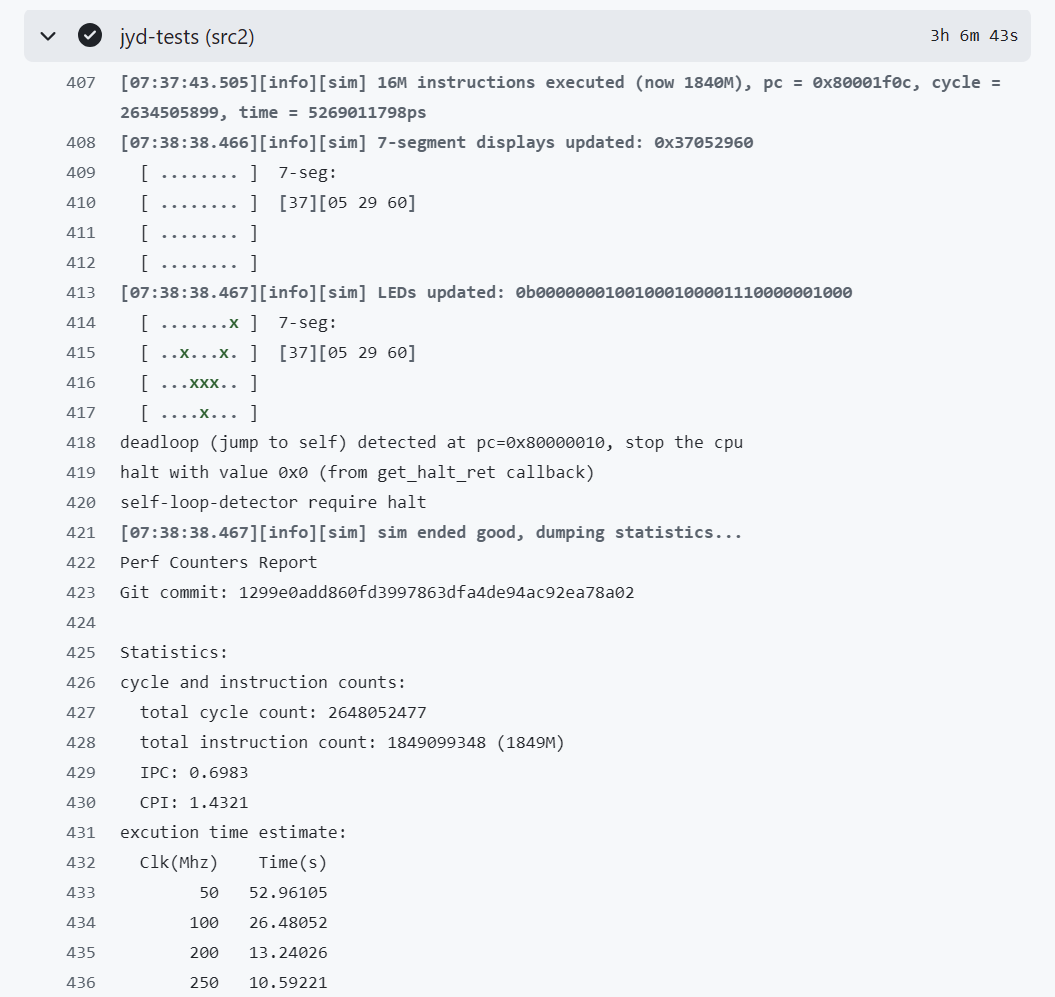
\includegraphics[width=0.84\linewidth,trim=0 340bp 0 0,clip]{image20.png}
  \caption{src2 仿真日志与性能统计结果}
\end{figure}

37 条指令测试通过。总周期数为 2,585,374,792，280 MHz 预测运行时间为 9.23348 s，
与实际上板测试结果 9.233 s 一致。

仿真性能计数器显示总周期数为 2585M，总动态指令数为 1849M，IPC 为 0.7152，CPI 为 1.3982。

\begin{figure}[H]
  \centering
  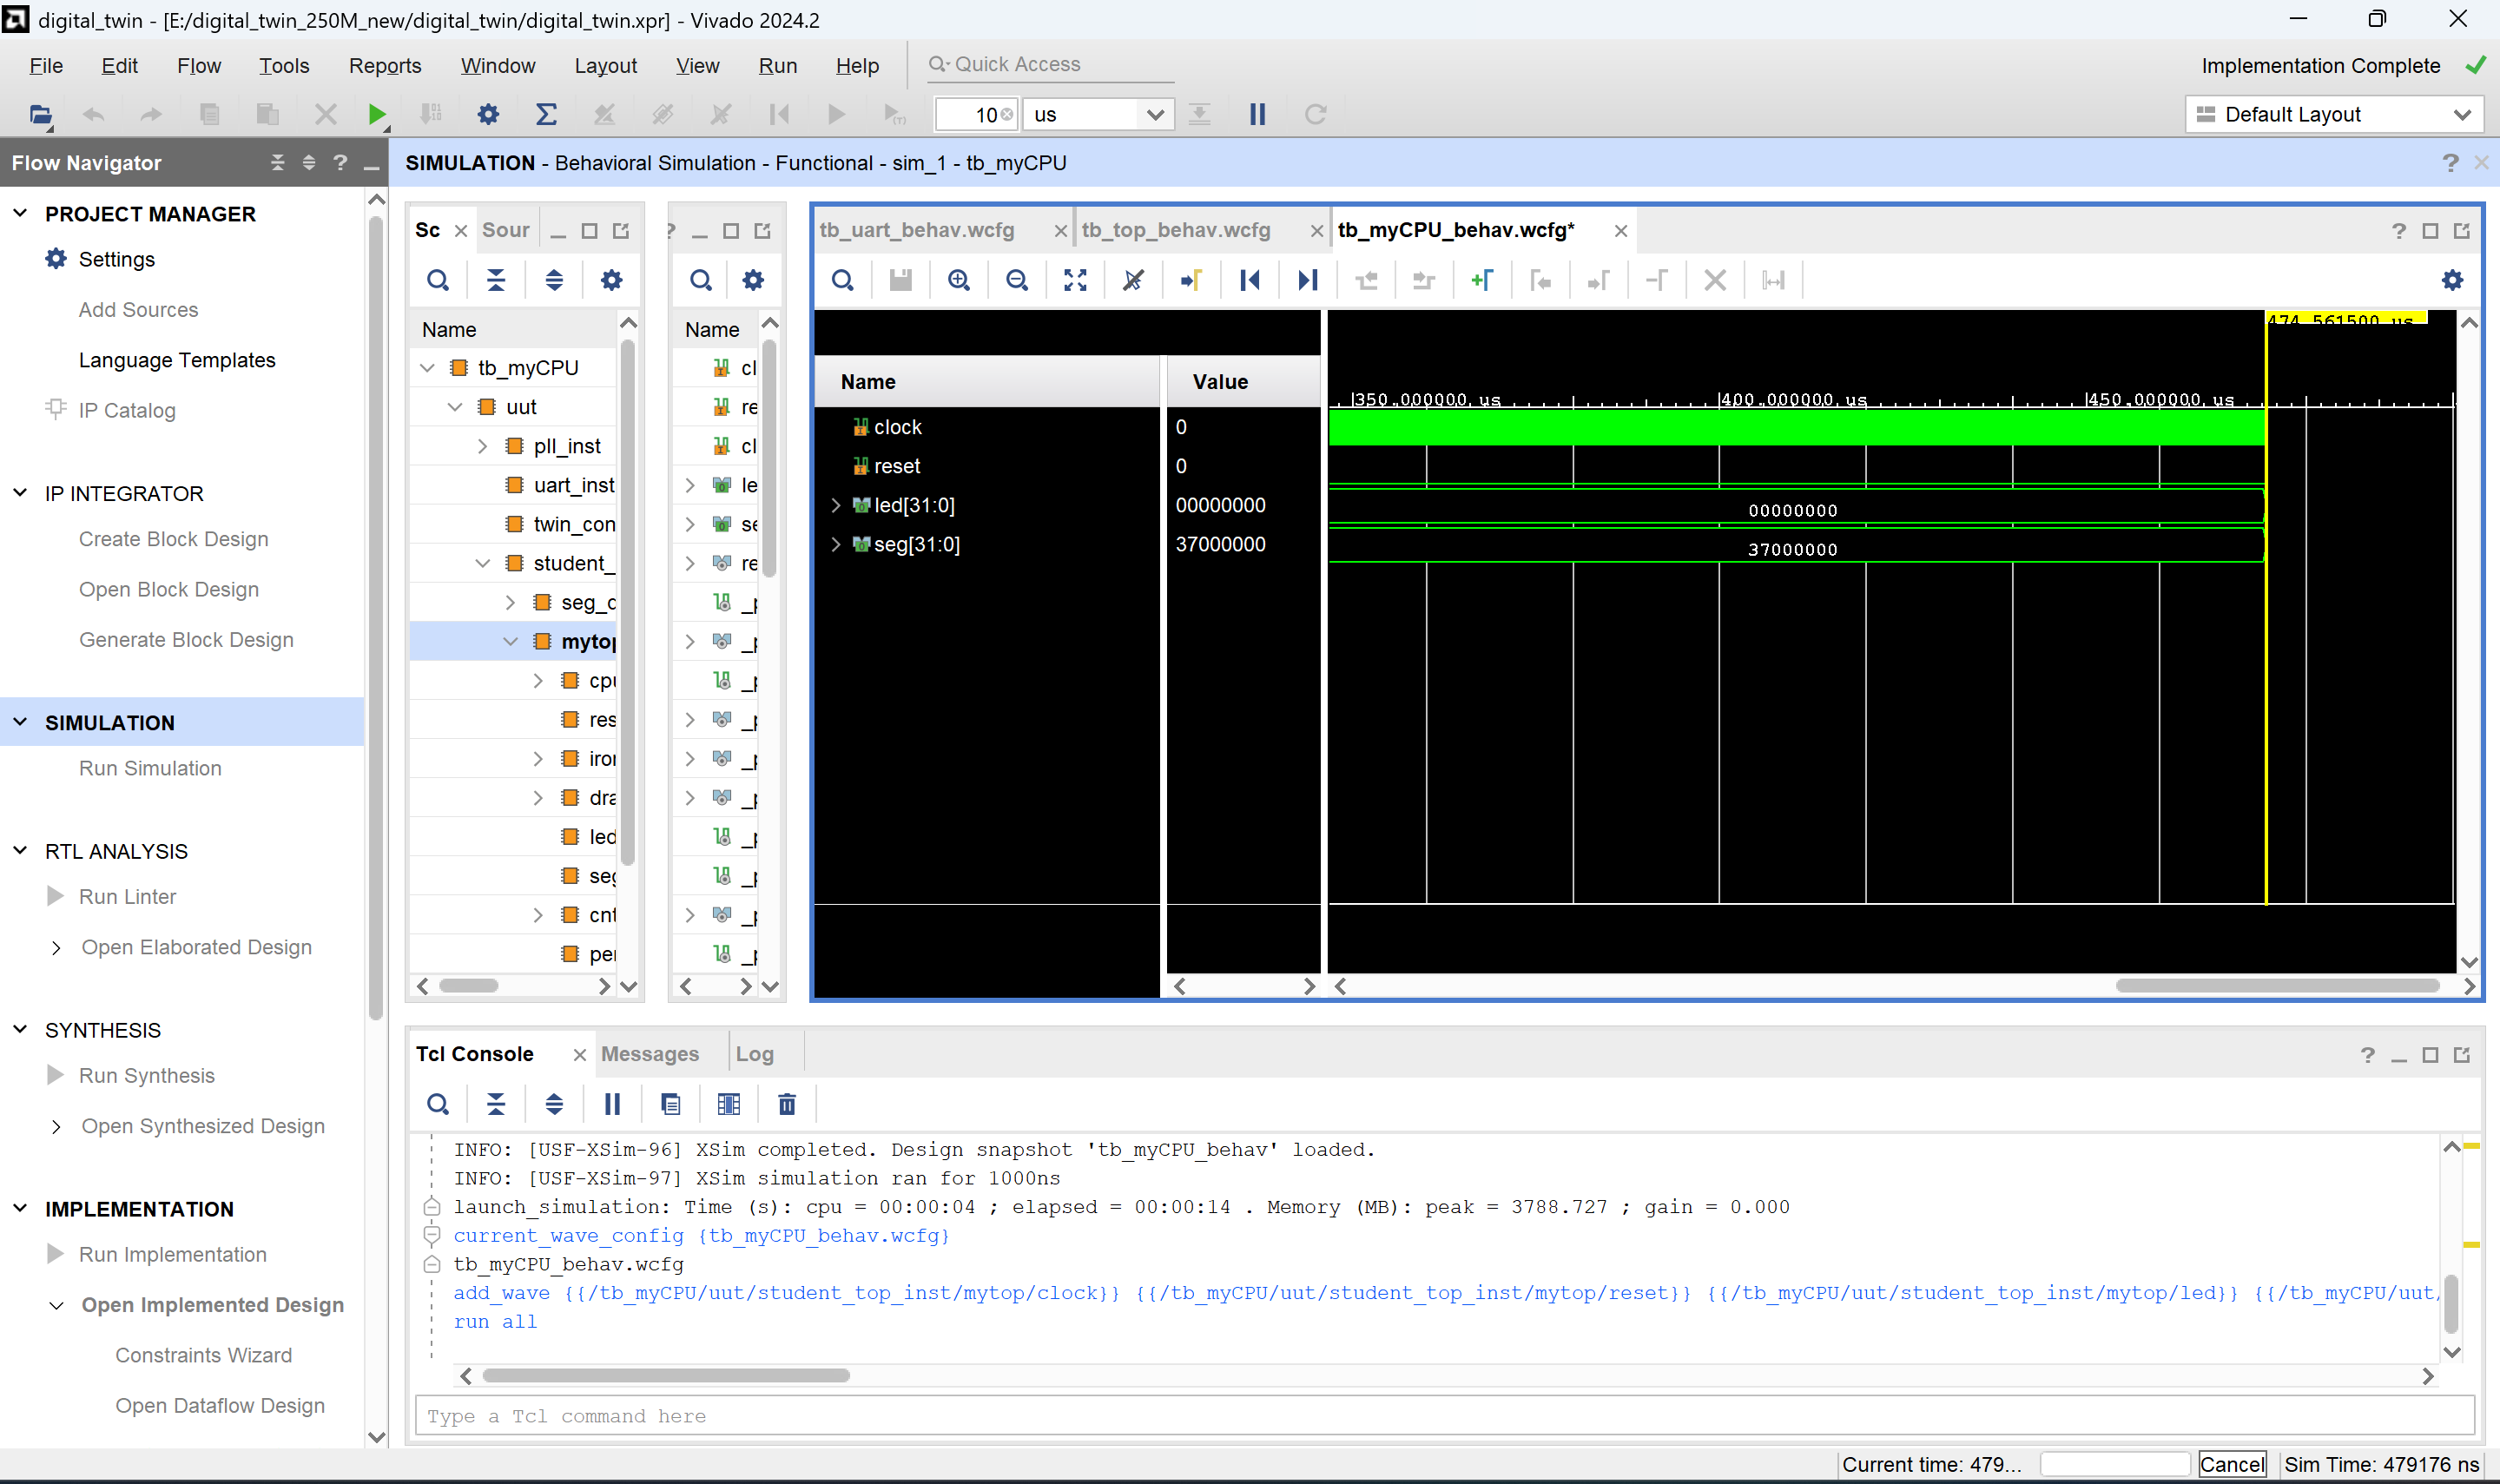
\includegraphics[width=\linewidth]{image21.png}
  \caption{src2 仿真波形结果}
\end{figure}

由图可知，数码管显示 37000000 证明 37 条指令测试正确通过。

\begin{threelongtable}{@{}
  C{0.12\linewidth}
  C{0.16\linewidth}
  C{0.16\linewidth}
  C{0.10\linewidth}
  C{0.10\linewidth}
  C{0.15\linewidth}@{}}
\caption{src0、src1、src2性能统计结果汇总}\\
\toprule
测试用例 & 总周期数 & 总指令数 & IPC & CPI & 280 MHz时间/s \\
\midrule
\endfirsthead
\toprule
测试用例 & 总周期数 & 总指令数 & IPC & CPI & 280 MHz时间/s \\
\midrule
\endhead
\bottomrule
\endlastfoot
src0 & 1988M & 1417M & 0.7130 & 1.4025 & 7.10133 \\
src1 & 1973M & 1304M & 0.6609 & 1.5131 & 7.04752 \\
src2 & 2585M & 1849M & 0.7152 & 1.3982 & 9.23348 \\
\end{threelongtable}

三组程序按周期数计算得到的 280 MHz 估算时间均与上板数码管显示结果一致。src2 的 IPC 最高、
CPI 最低；src1 的 CPI 相对较高，但相比初赛版本已有明显改善。

\subsubsection{coremark 性能测试用例}

\begin{figure}[H]
  \centering
  % 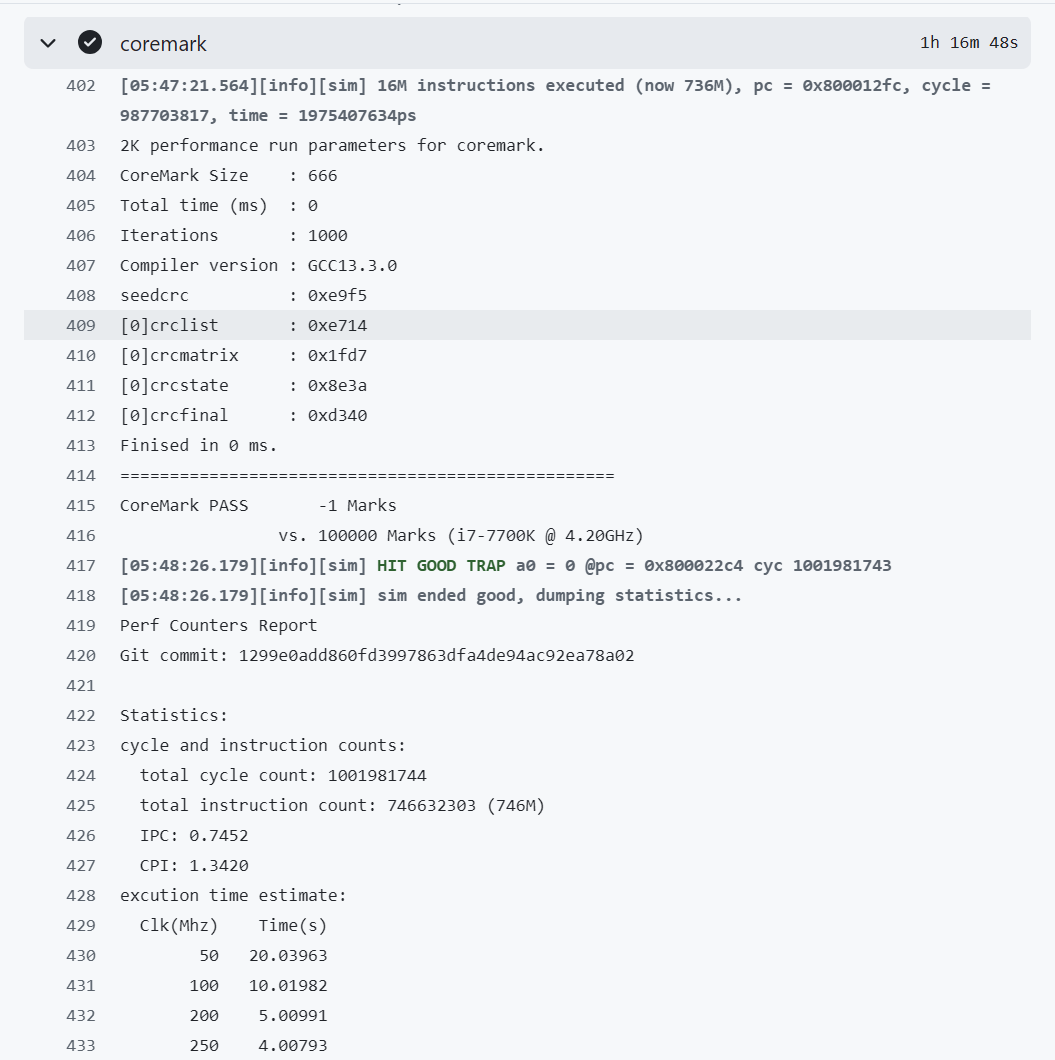
\includegraphics[width=0.45\linewidth]{image22.png}\hfill
  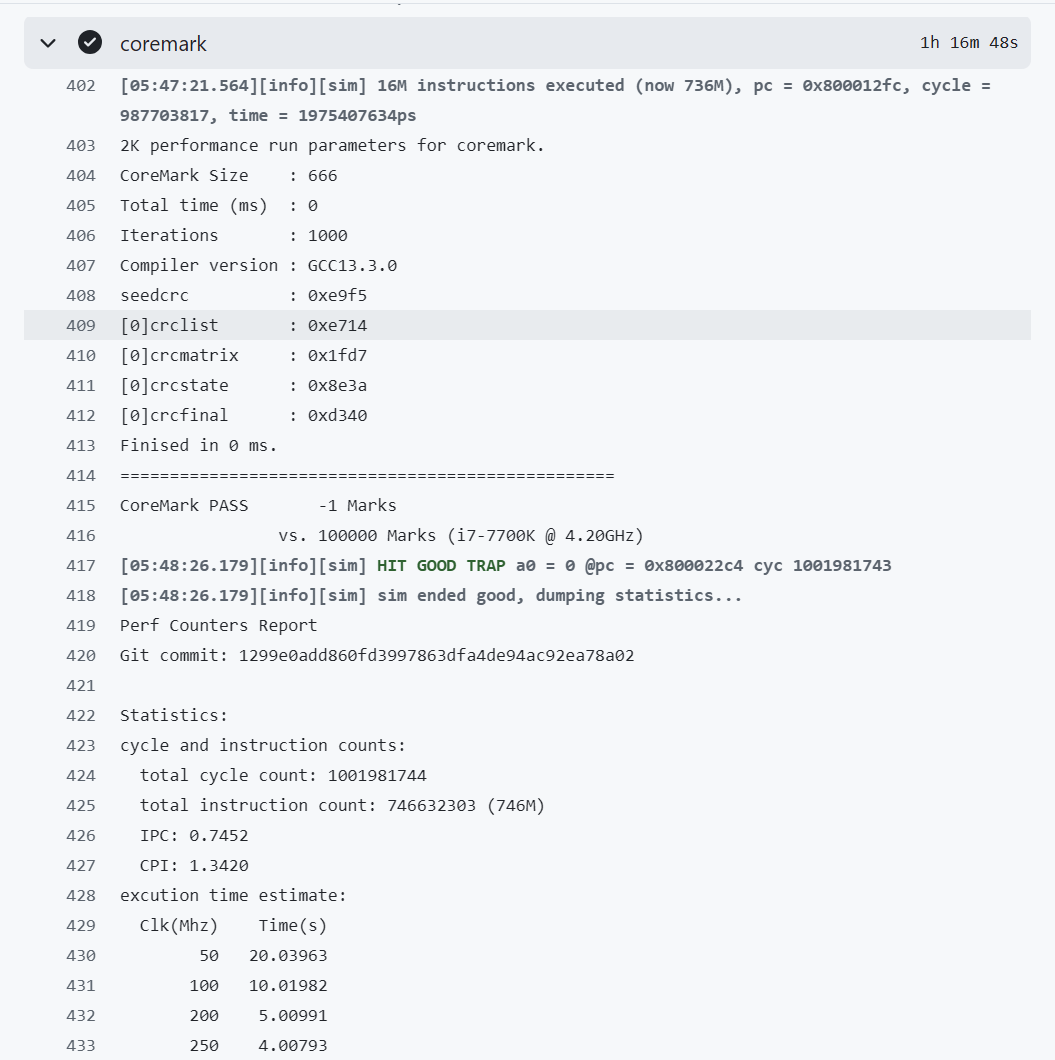
\includegraphics[width=0.82\linewidth,trim=0 440bp 0 0,clip]{image22.png}
  \caption{coremark 测试结果截图}
\end{figure}

本次 CI 完成 1000 次迭代，共执行 472,993,621 周期，IPC 为 0.6625、CPI 为 1.5094。
按 280 MHz 计算运行时间为 1.68926 s，CI 输出的 CoreMark 结果为 308：

\[
  \text{CoreMark} = 308
\]

或者归一化：

\[
  \text{CoreMark/MHz} = \frac{308}{280} = 1.10
\]

达到基础顺序执行处理器的预期水平。

\subsubsection{dhrystone 性能测试用例}

\begin{figure}[H]
  \centering
  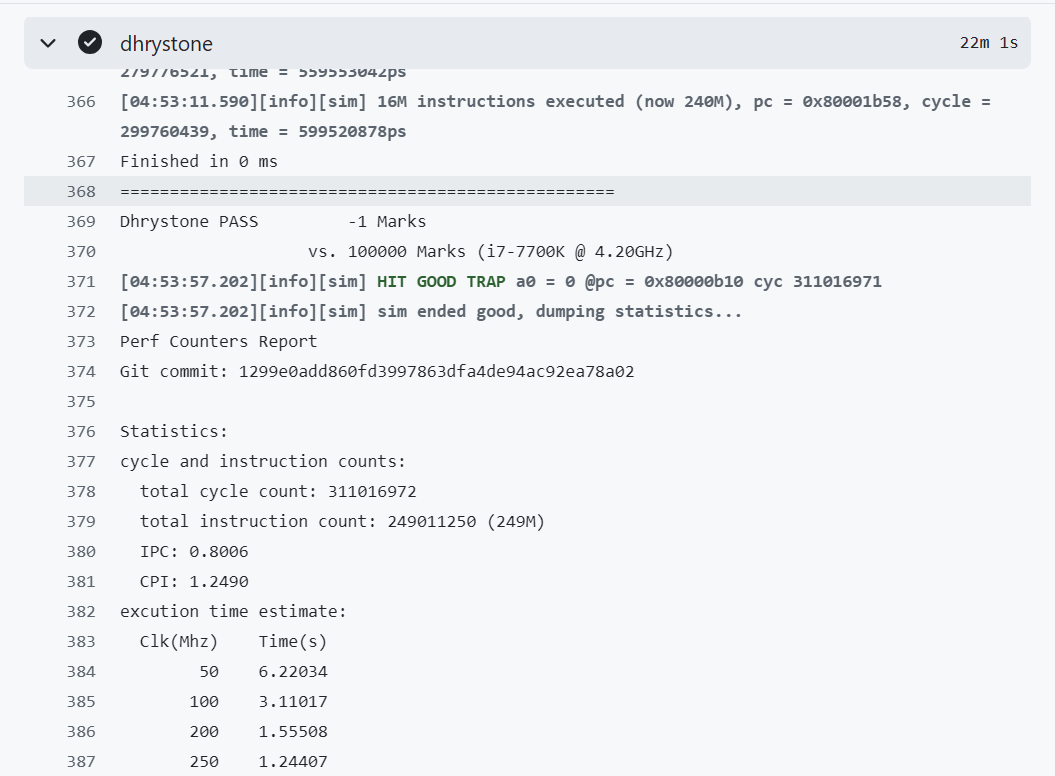
\includegraphics[width=0.82\linewidth,trim=0 545bp 0 0,clip]{image23.png}
  \caption{dhrystone 测试结果截图}
\end{figure}

CPI 为 1.2873（IPC 为 0.7768），总周期数为 302,517,149；按 280 MHz 计算，
500000 次迭代的估算时间为 1.08042 s：

\[
  \text{Dhrystones/s} = \frac{\text{NUMBER\_OF\_RUNS}}{\text{Time}}
\]

\[
  \frac{500000}{1.080418389} \approx 462783.69\text{~Dhrystones/s}
\]

DMIPS 公式：

\[
  \text{DMIPS} = \frac{\text{Dhrystones/s}}{1757} \approx 263.39
\]

归一化：

\[
  \text{DMIPS/MHz} = \frac{263.39}{280} \approx 0.941
\]

达到基础顺序执行处理器的预期水平。

\subsection{RV32I CPU其他测试结果}

下面的图片展示了在 RT-Thread 上运行 version、free 等基础指令以及嵌入的 hello 和 microbench 程序。

\begin{figure}[H]
  \centering
  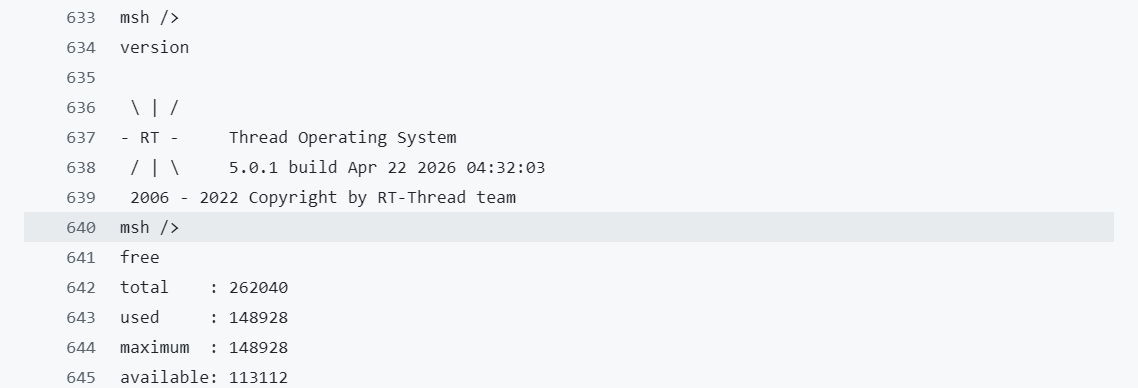
\includegraphics[width=\linewidth]{image24.png}
  \vspace{0.3em}
  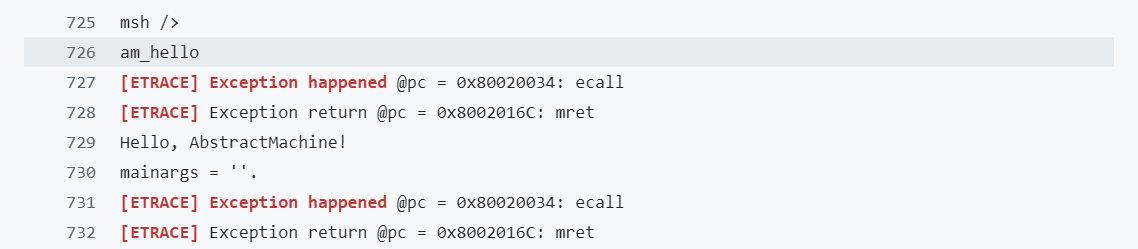
\includegraphics[width=\linewidth]{image25.png}
  \vspace{0.3em}
  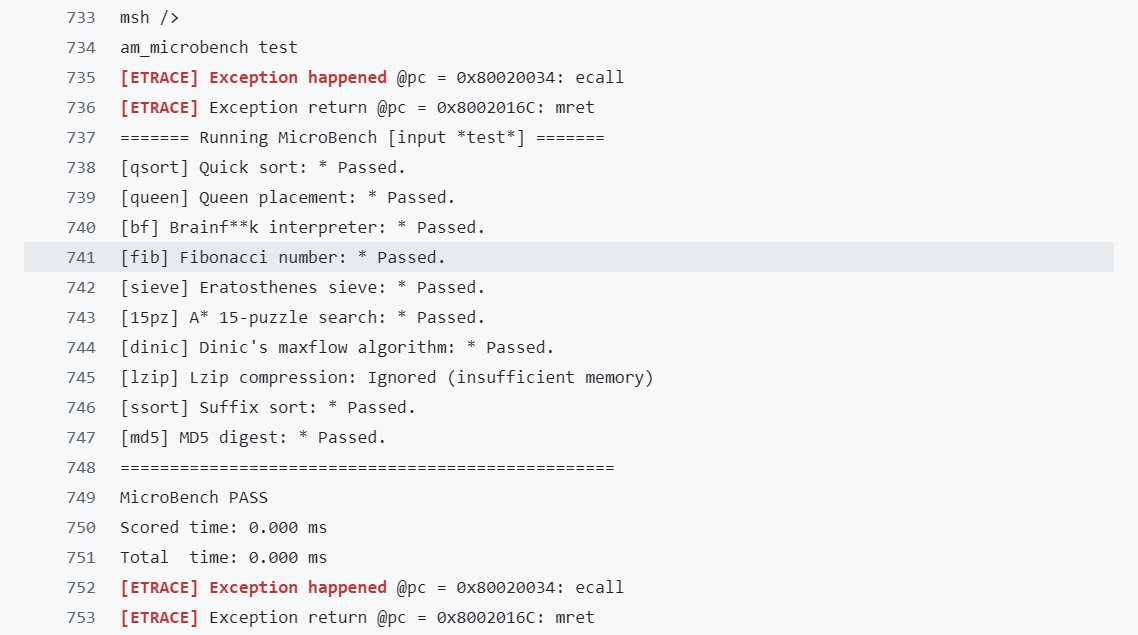
\includegraphics[width=\linewidth]{image26.png}
  \vspace{0.3em}
  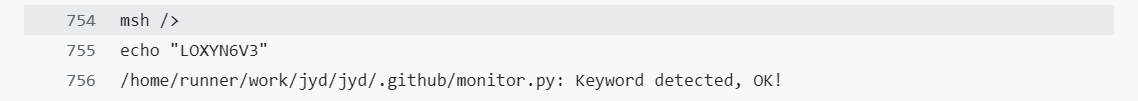
\includegraphics[width=\linewidth]{image27.png}
  \caption{RT-Thread 自动化测试输出节选}
\end{figure}

最后的 echo 测试输出了预期的随机字符串，从而使 monitor 认为行为正确直接结束了测试，没有将其输出回放到 CI 的标准输出。综上表明仿真环境运行正常，CI 测试通过。

\begin{figure}[H]
  \centering
  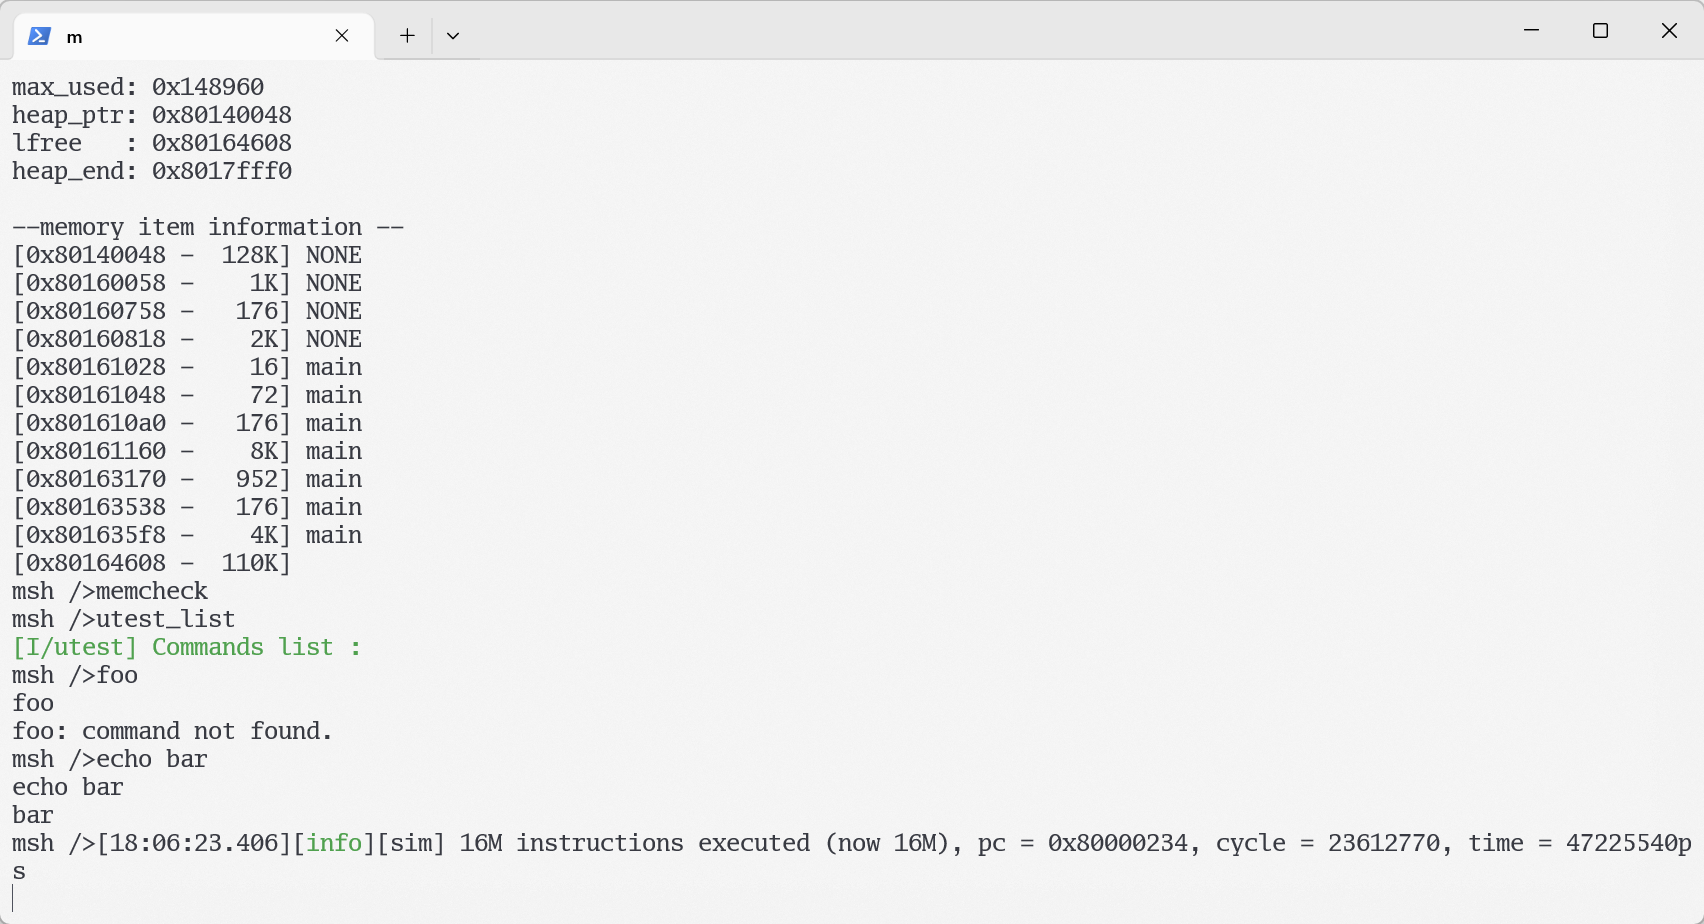
\includegraphics[width=0.9\linewidth]{image28.png}
  \caption{RT-Thread 本地交互测试}
\end{figure}

本地环境通过仿真串口输入进行测试，行为符合预期，测试通过。

\newpage

\section{仿真总结}

本章围绕自研 RV32I CPU 进行了仿真工作。项目采用了 Vivado Simulation 与 Verilator/C++ 两类仿真平台。

在功能正确性验证方面，本项目针对 RV32I 基本整数指令集进行了单指令测试与小规模程序测试，覆盖了算术逻辑运算、立即数运算、访存访问、条件分支、跳转等典型执行路径。仿真结果表明，CPU 能够正确执行 RV32I 基本指令且能够处理相关边界样例。项目还通过 DPI-C 实现了 EBREAK 停机检测、LED/SEG 外设的软件侧模拟，并引入软件 RISC-V 模拟器作为差分测试参考模型。

在性能测评方面，项目对官方 src0、src1、src2 三组性能测试用例进行了完整仿真，并通过性能计数器
统计周期数、指令数、IPC 和 CPI。统计结果显示，三组程序的 CPI 分别为 1.4025、1.5131 和
1.3982，280 MHz 估算时间分别为 7.10133 s、7.04752 s 和 9.23348 s，与上板结果一致。
此外，项目完成了 CoreMark 和 Dhrystone 测试；CoreMark 为 308，CoreMark/MHz 为 1.10，
Dhrystone 估算为 462783.69 Dhrystones/s、DMIPS/MHz 约为 0.941。

在扩展软件运行能力方面，本项目支持了部分 CSR 寄存器以及 ecall、mret、csrrw、csrrs 等机制，并完成了面向 RT-Thread 测试的基础适配。仿真环境能够通过串口输入运行 version、free、hello、microbench 等基础测试命令，自动化测试和本地交互测试均表现正常。该部分结果说明本项目已经具备运行更复杂软件负载的基础能力，为后续扩展异常中断处理、操作系统支持和更完整的软件生态验证提供了条件。

综上，本项目已经完成了指令级单元测试、程序级测试、官方性能测试、通用 benchmark 和 RT-Thread 运行测试。相比单纯依赖波形观察的验证方式，本项目的主要亮点在于构建了自动化、可差分、可量化、可持续集成的 CPU 仿真验证体系，并通过性能计数器对 CPI、IPC、分支预测准确率和数据相关阻塞等指标进行了细粒度分析。上述结果表明，本项目 CPU 在 RV32I 功能正确性、仿真验证完整性、性能可观测性和软件运行扩展性方面均达到了较好的完成度。

\end{document}
